
% Chapter 

%\chapter{Quantitative Analysis of Thesis reflexivity}{Analyse de la réflexivité} % Chapter title
\chapter{Analyse Reflexive}


\markboth{\thechapter\space Réflexivité}{\thechapter\space Réflexivité}


\label{app:reflexivity} % For referencing the chapter elsewhere, use \autoref{ch:name} 

%----------------------------------------------------------------------------------------

%  ``Meta-conclusion''
%  -> should also include reading graph / possible paths



% To clarify the plan : Plan (of course) ; diagram for plan ; and dependence tree for parts/sections





%%%%%%%%%%%%
\subsection{Hypernetwork analysis}{Analyse par hyperréseau}






%%%%%%%%%%%%
\begin{figure}
	%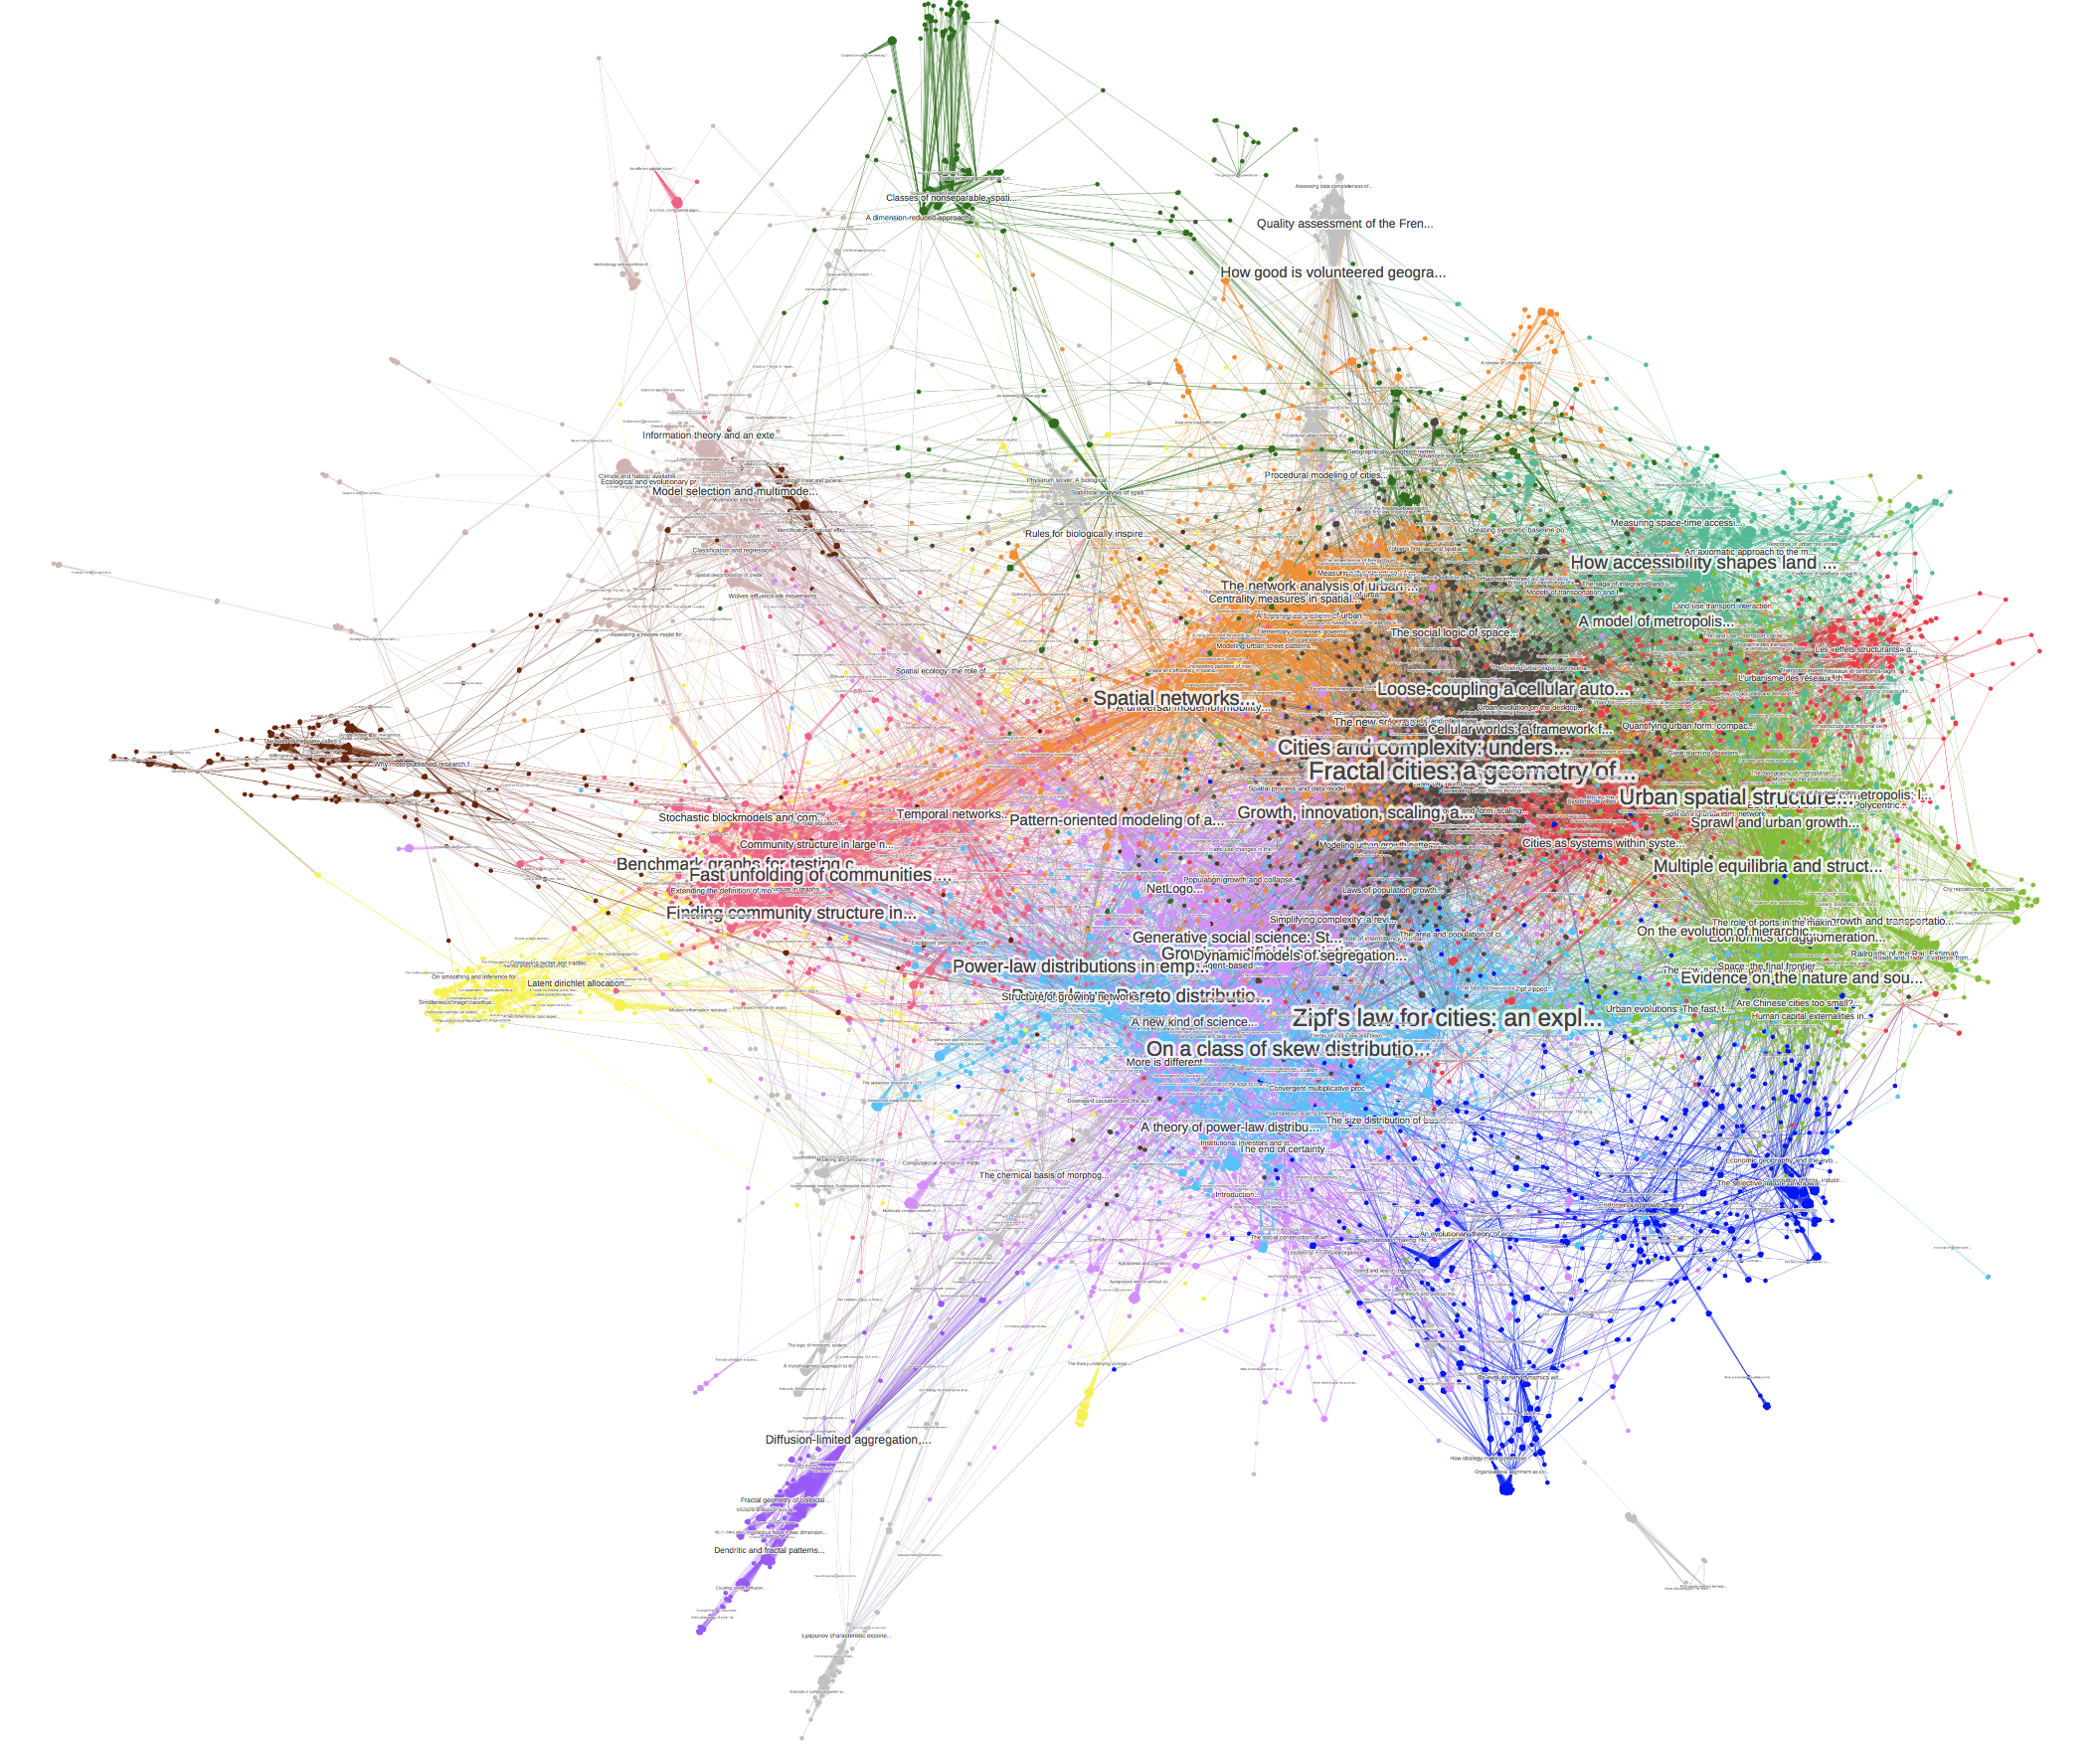
\includegraphics[width=\textwidth]{Figures/Reflexivity/citcore.png}
	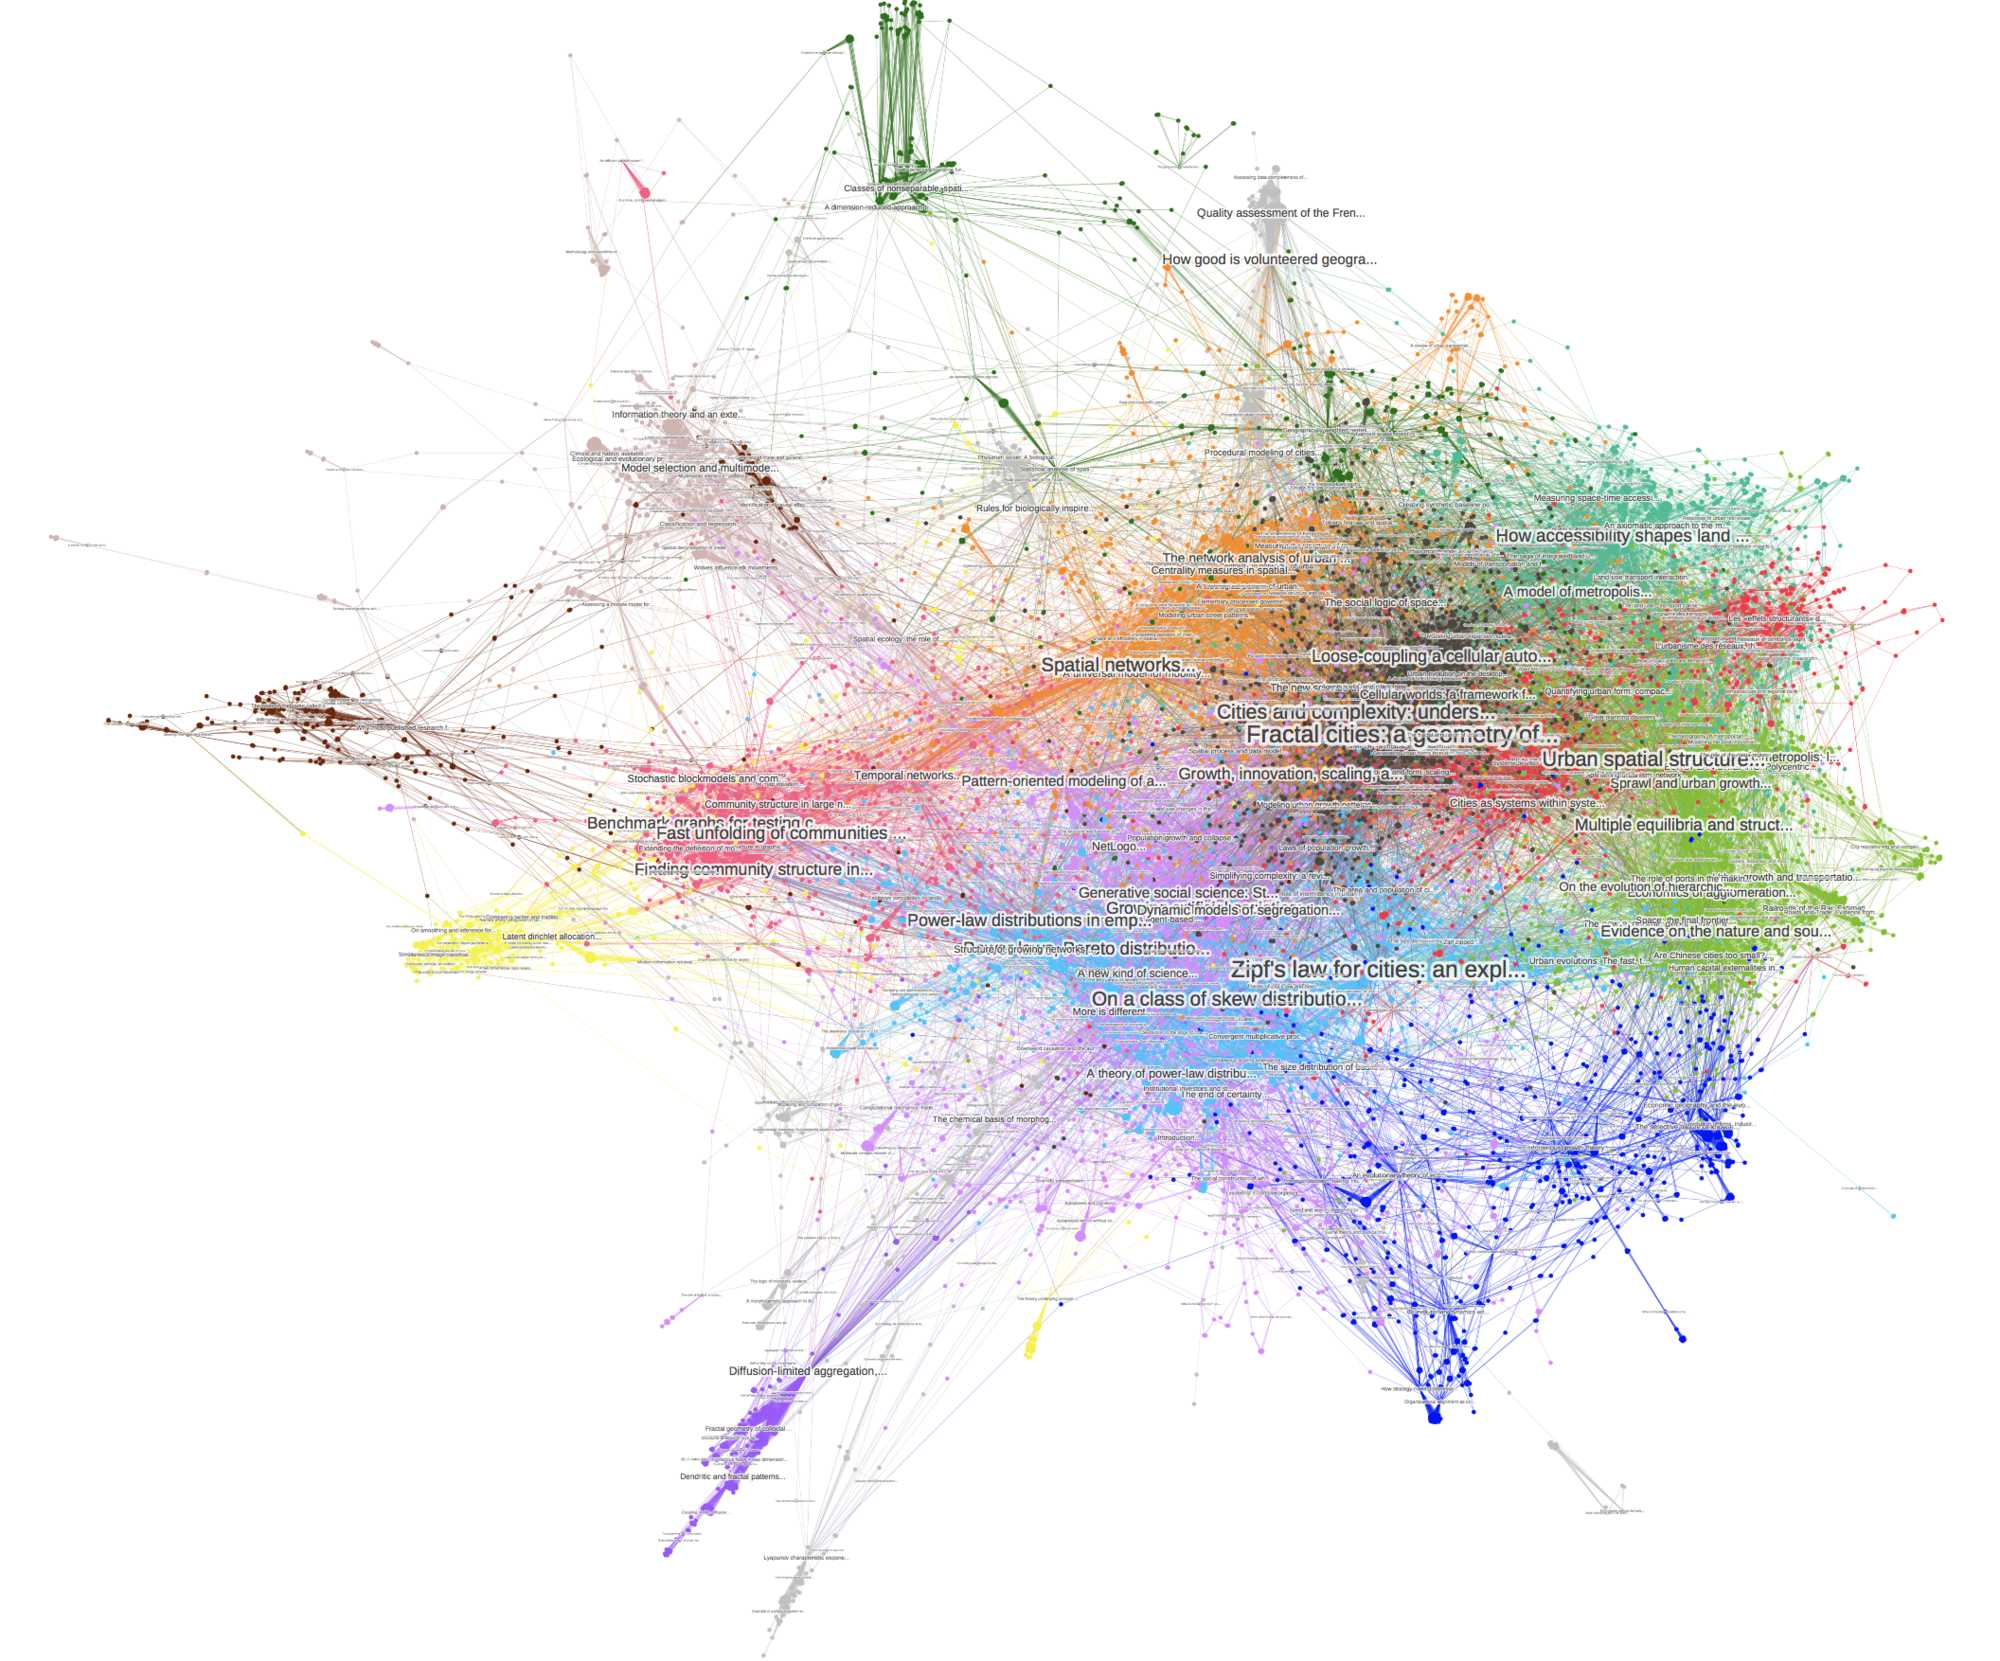
\includegraphics[width=\linewidth]{Figures/Final/F-reflexivity-citnw.jpg}
	\appcaption{\textbf{Citation network.}\label{fig:app:reflexivity:citnw}}{\textbf{Réseau de citation.}\label{fig:app:reflexivity:citnw}}
\end{figure}
%%%%%%%%%%%%









%%%%%%%%%%%%
\subsection{Interaction between projects}{Interaction entre projets}




%%%%%%%%%%%%
\begin{figure}
	%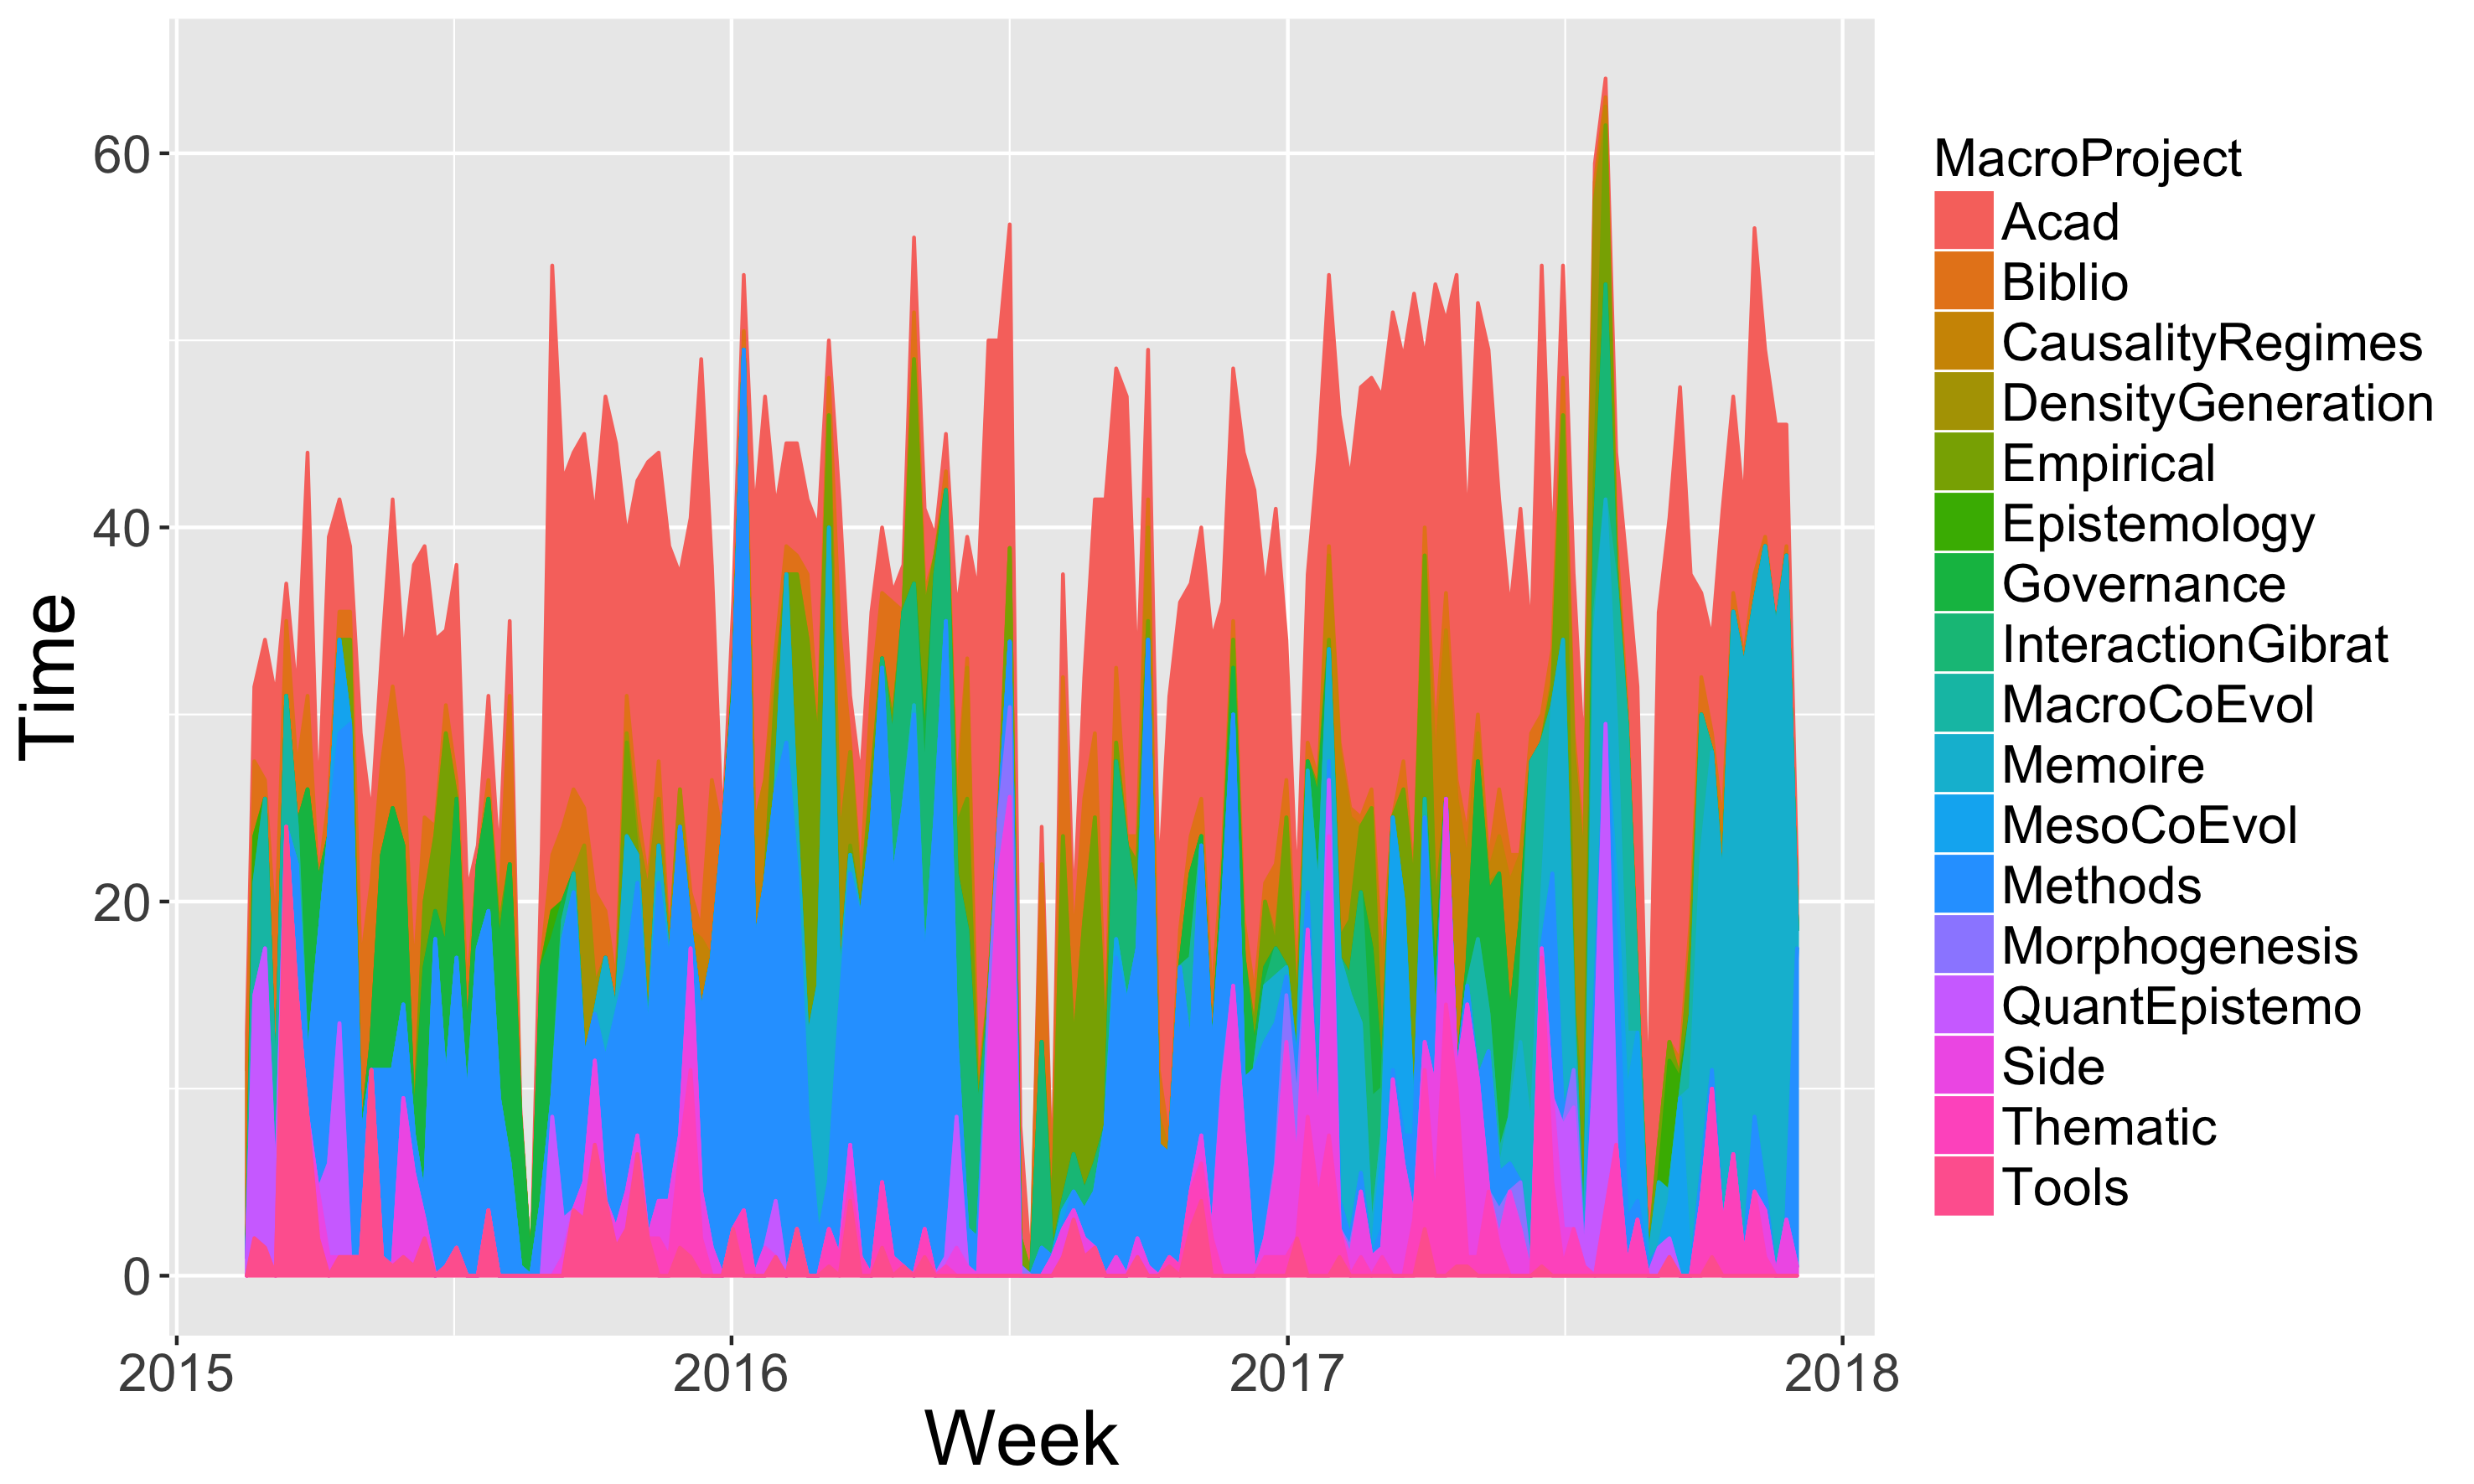
\includegraphics[width=\linewidth]{Figures/Reflexivity/weekly-macroproj.png}
	%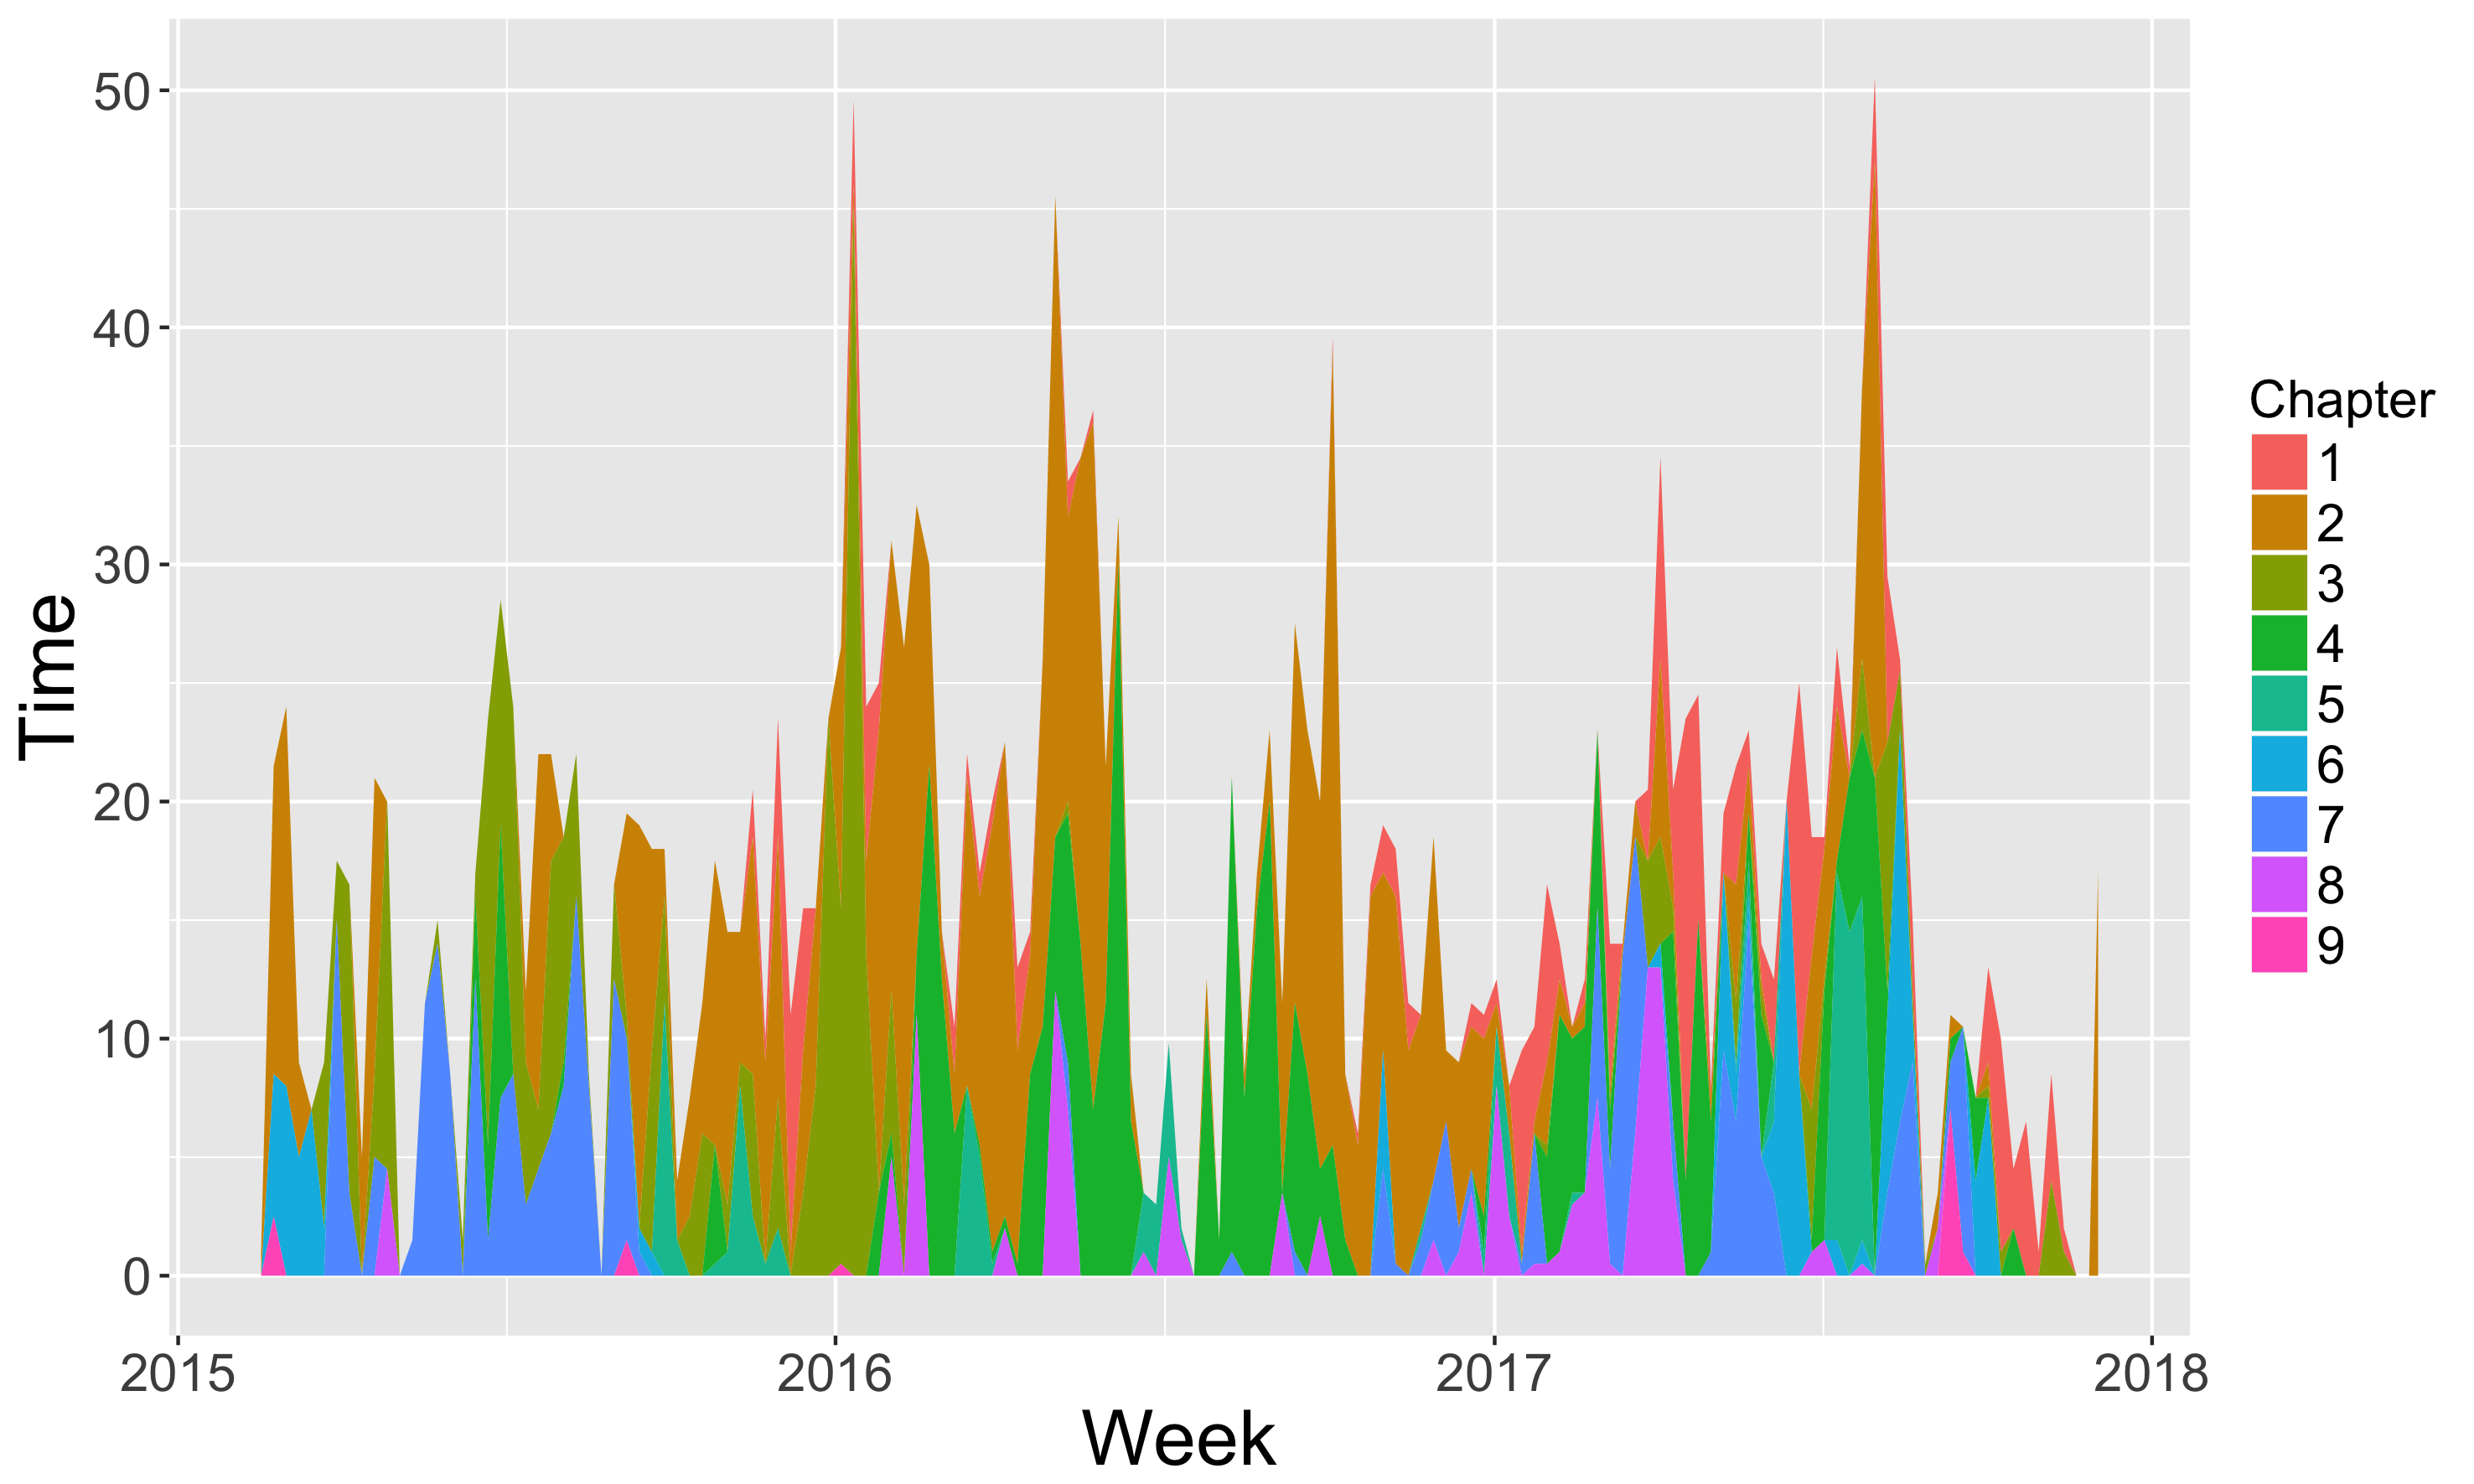
\includegraphics[width=\linewidth]{Figures/Reflexivity/weekly-chapter.png}
	%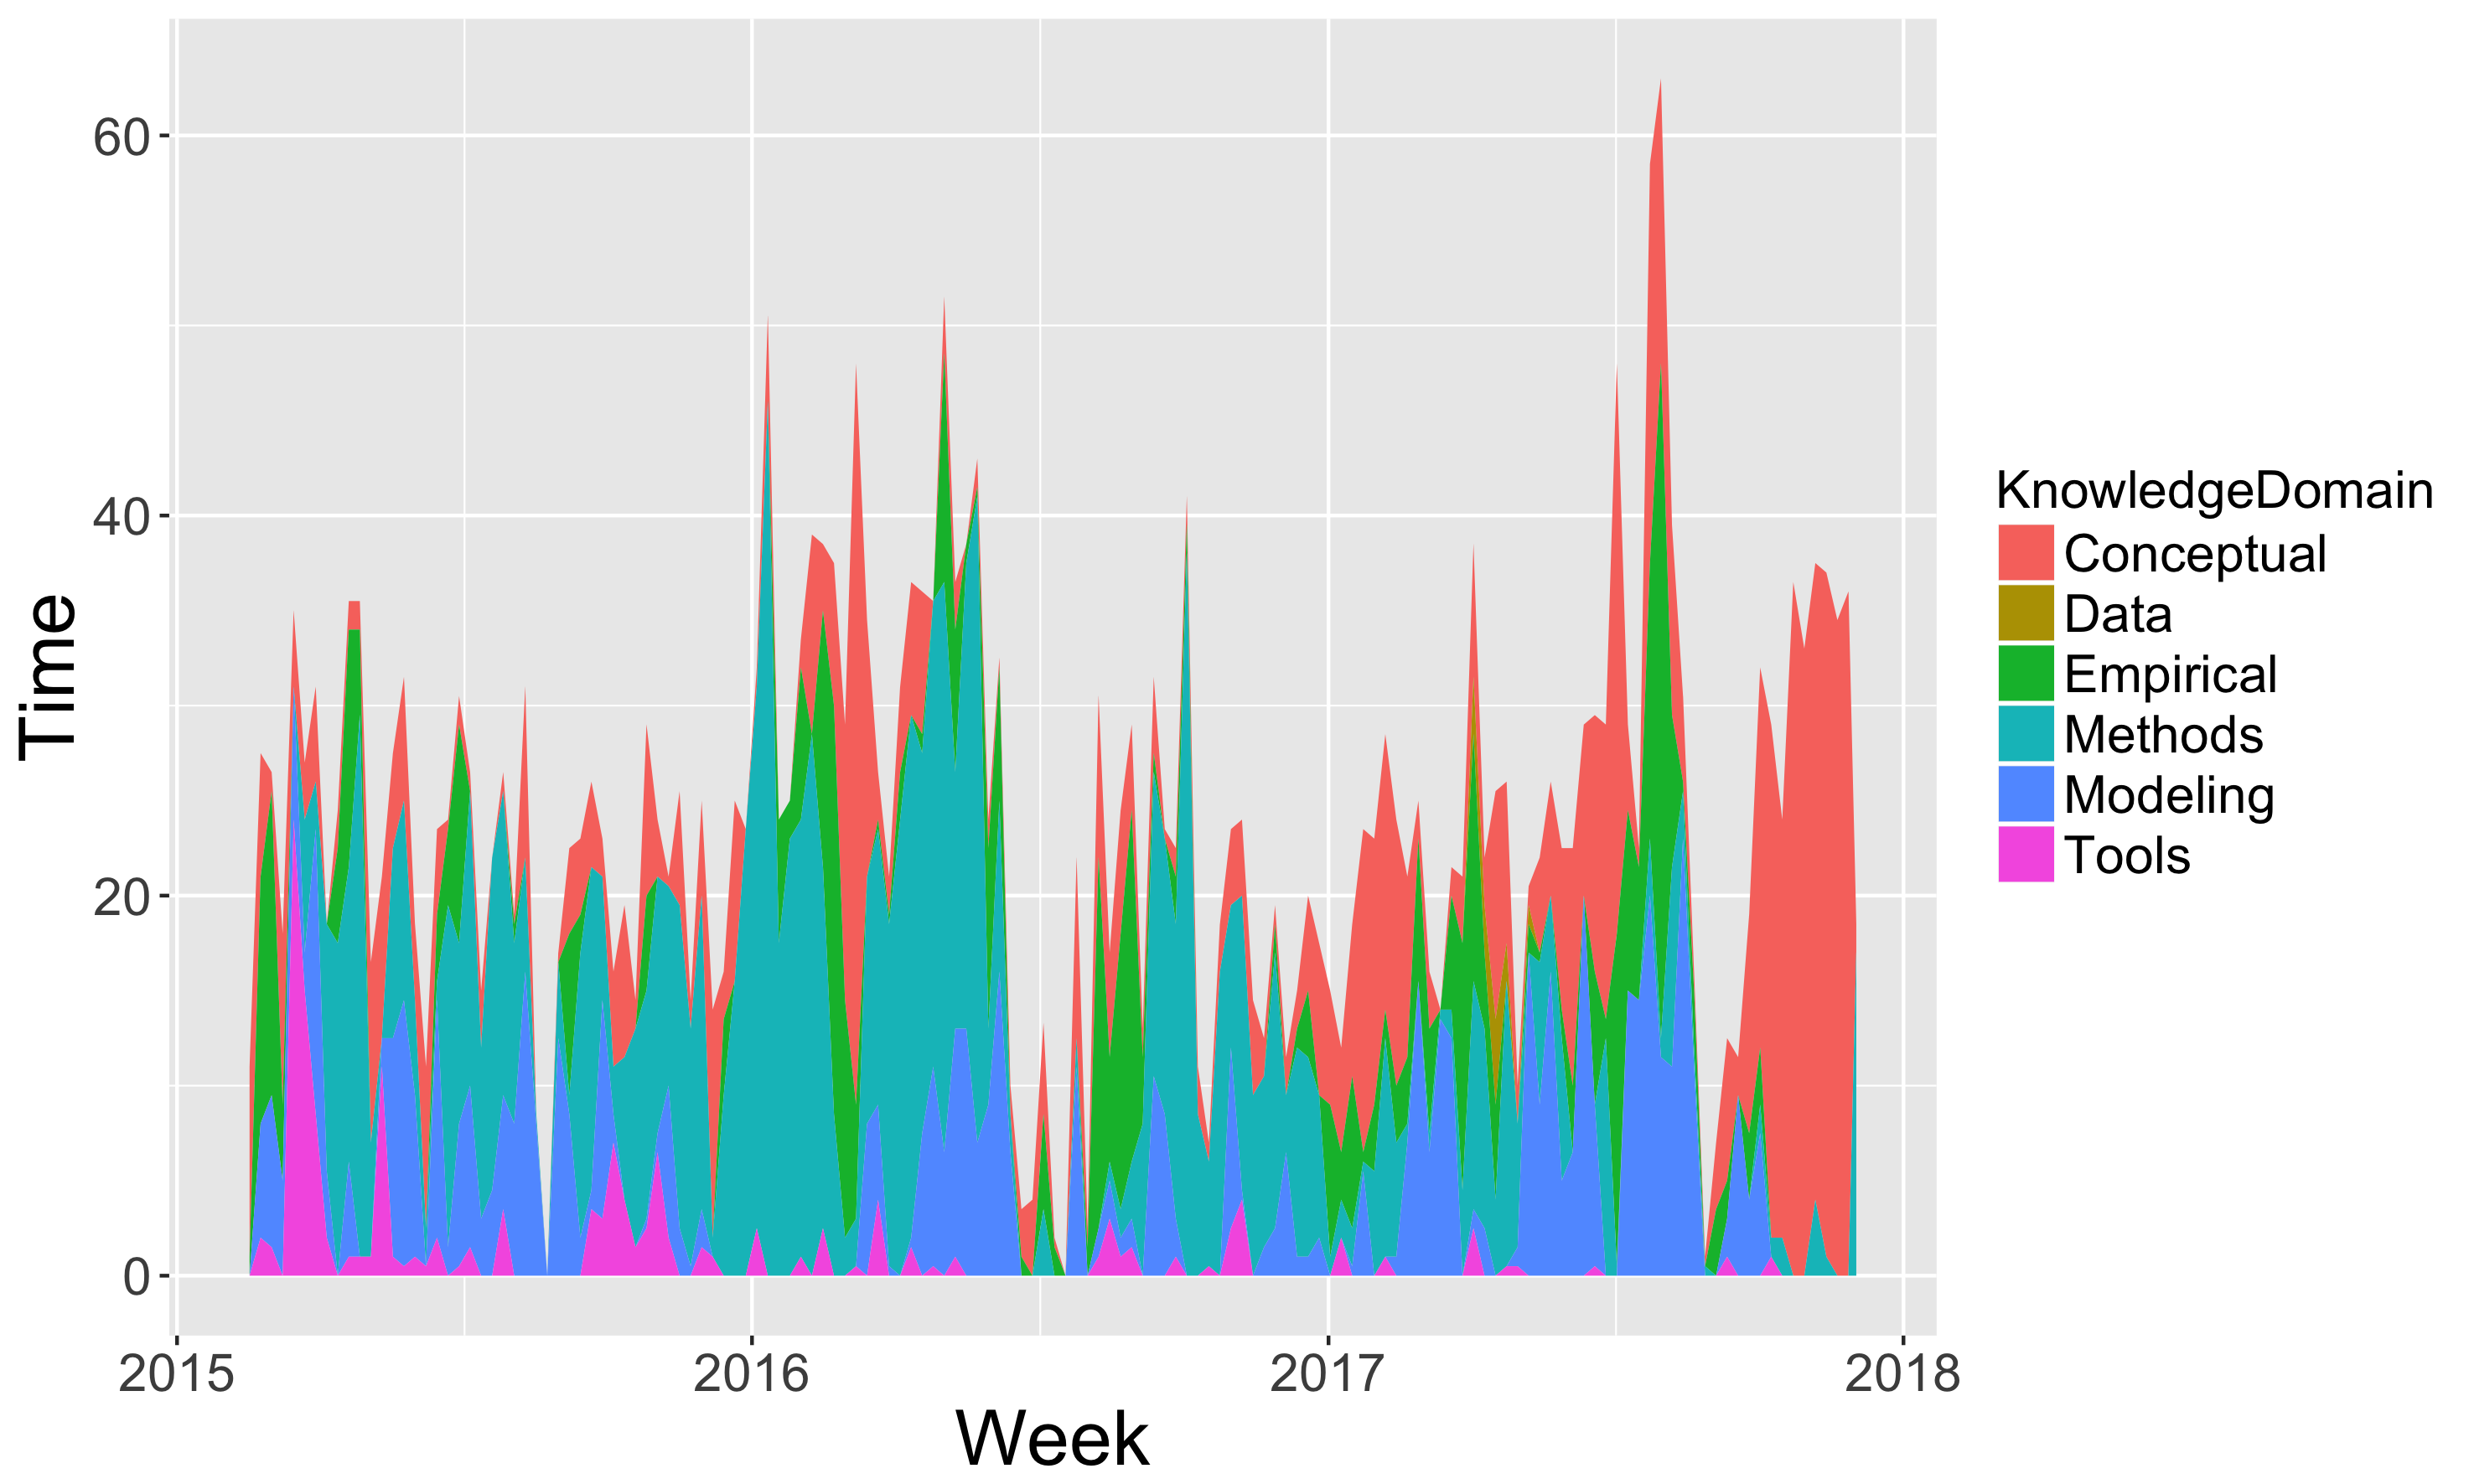
\includegraphics[width=\linewidth]{Figures/Reflexivity/weekly-knowledgedomains.png}
	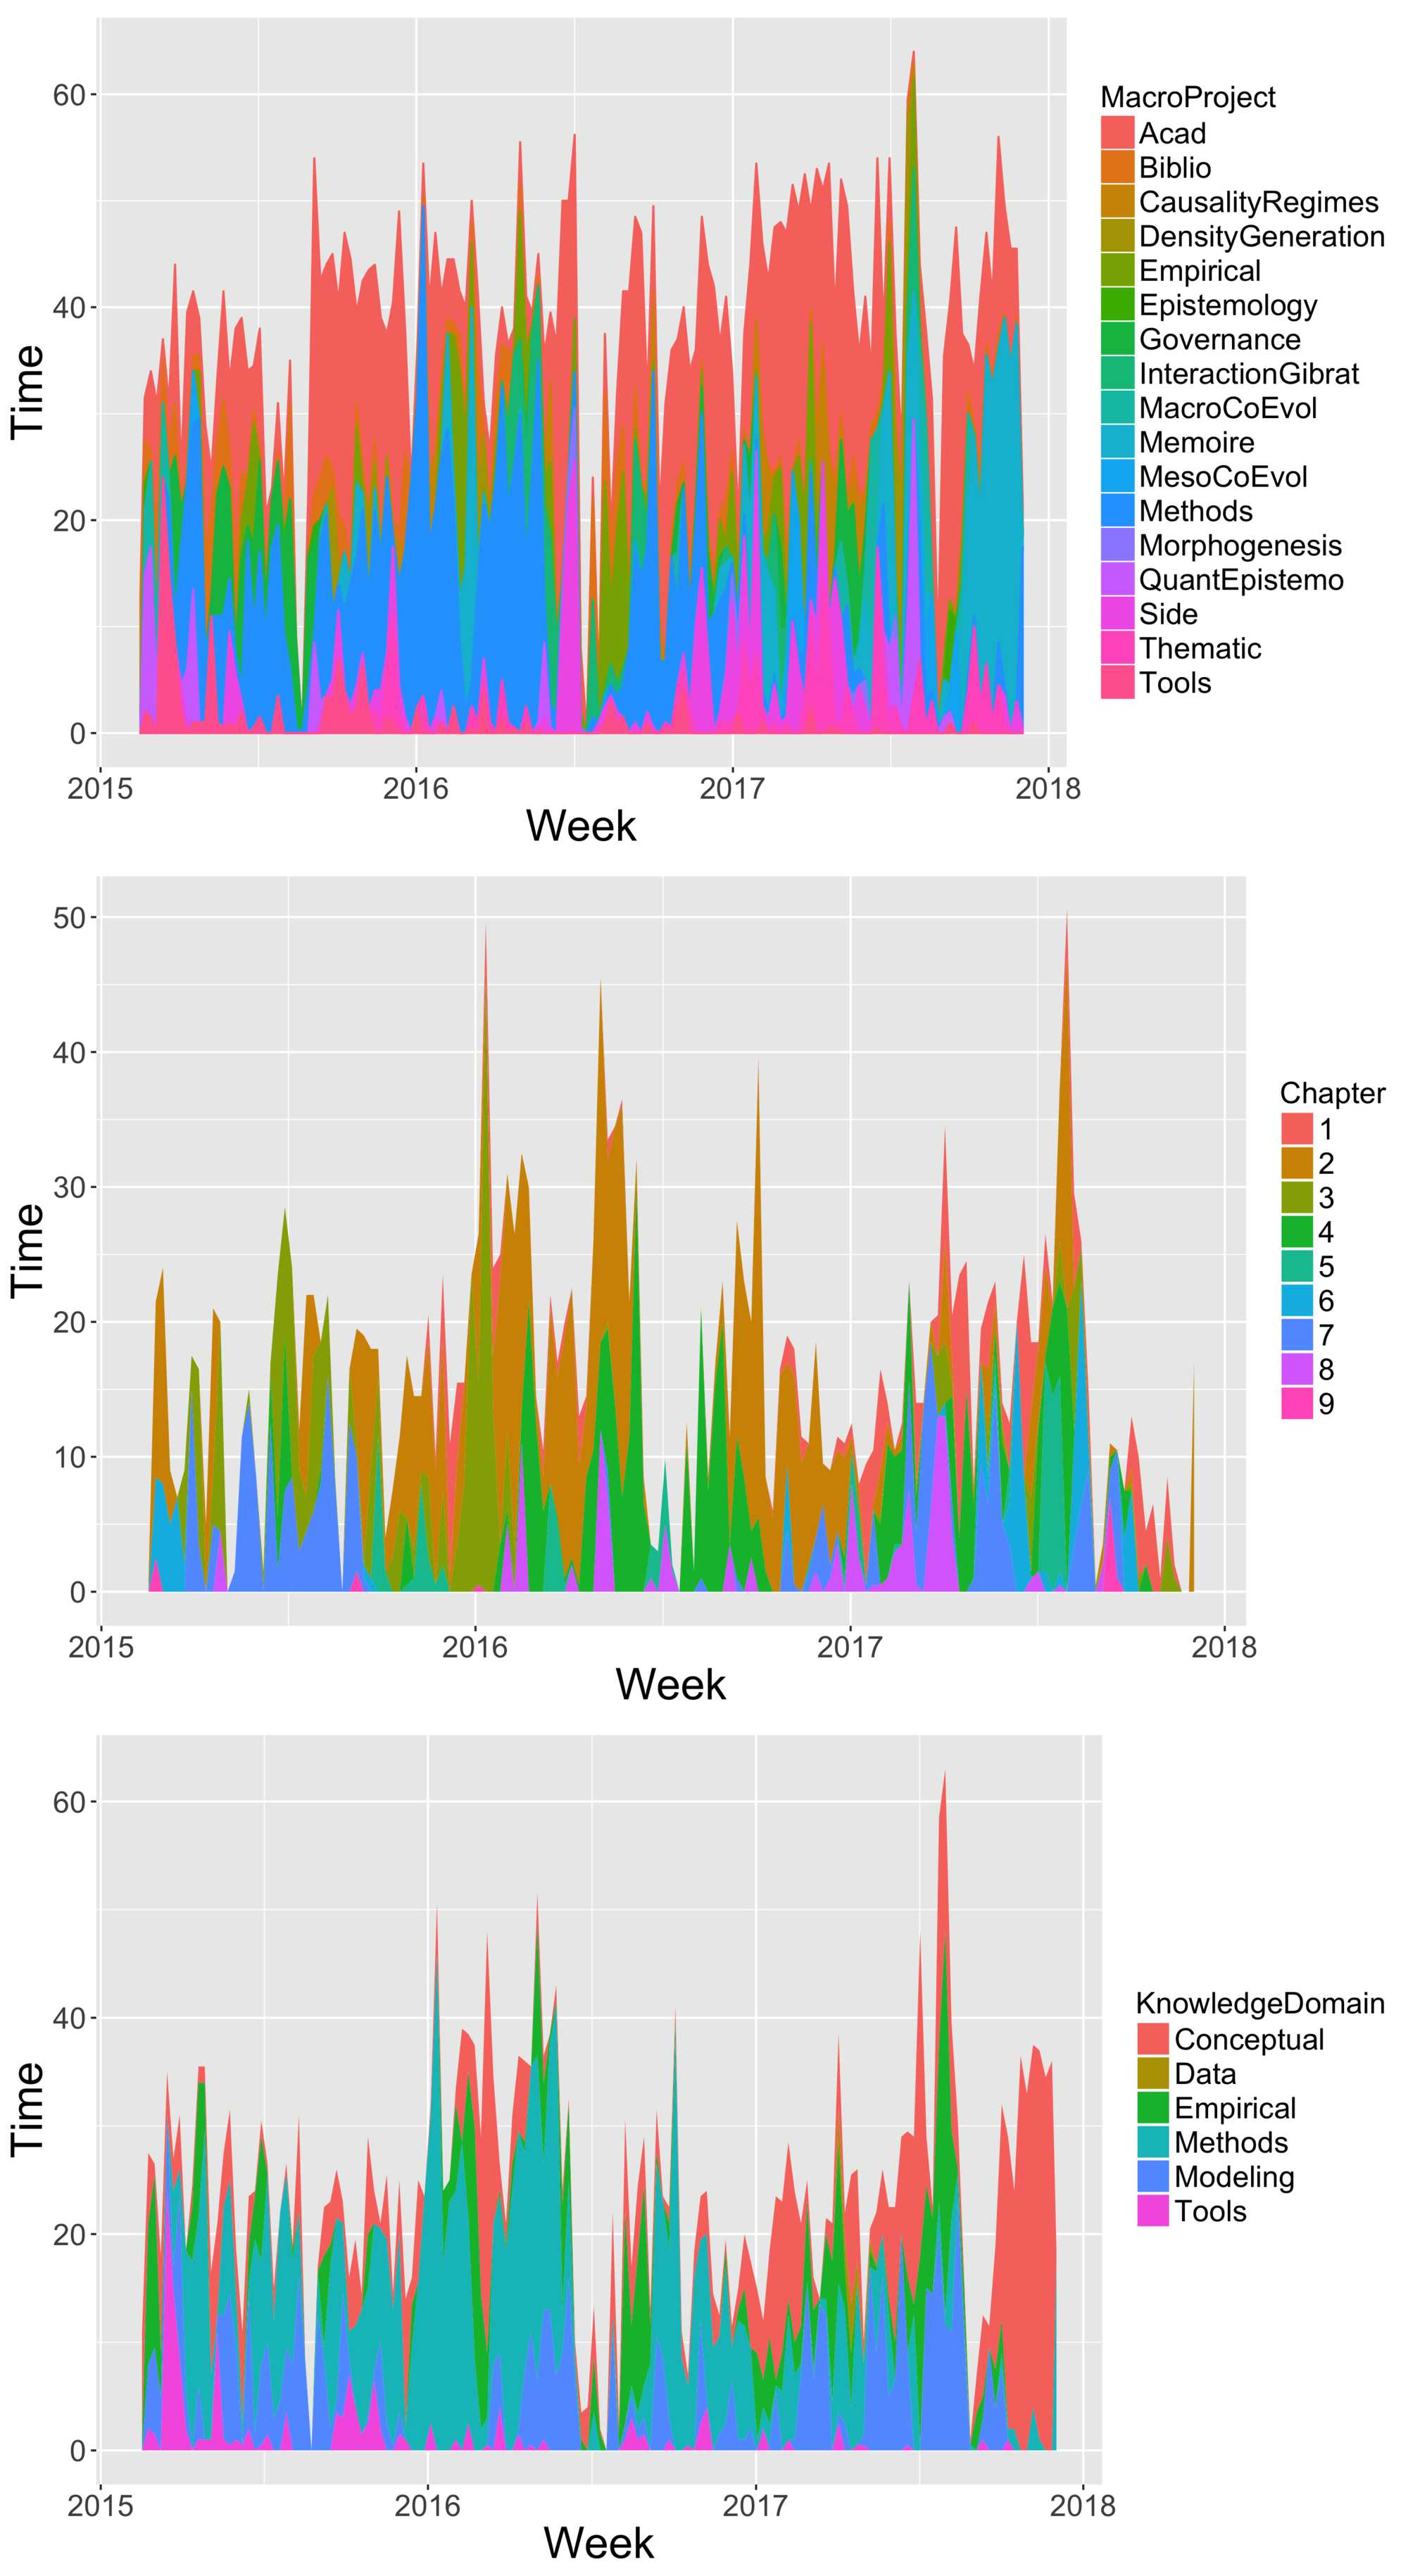
\includegraphics[width=\textwidth]{Figures/Final/F-reflexivity-time.jpg}
	\appcaption{\textbf{Temporal distribution.}\label{fig:app:reflexivity:time}}{\textbf{Répartition temporelle.}\label{fig:app:reflexivity:time}}
\end{figure}
%%%%%%%%%%%%



%%%%%%%%%%%%
\begin{figure}
	%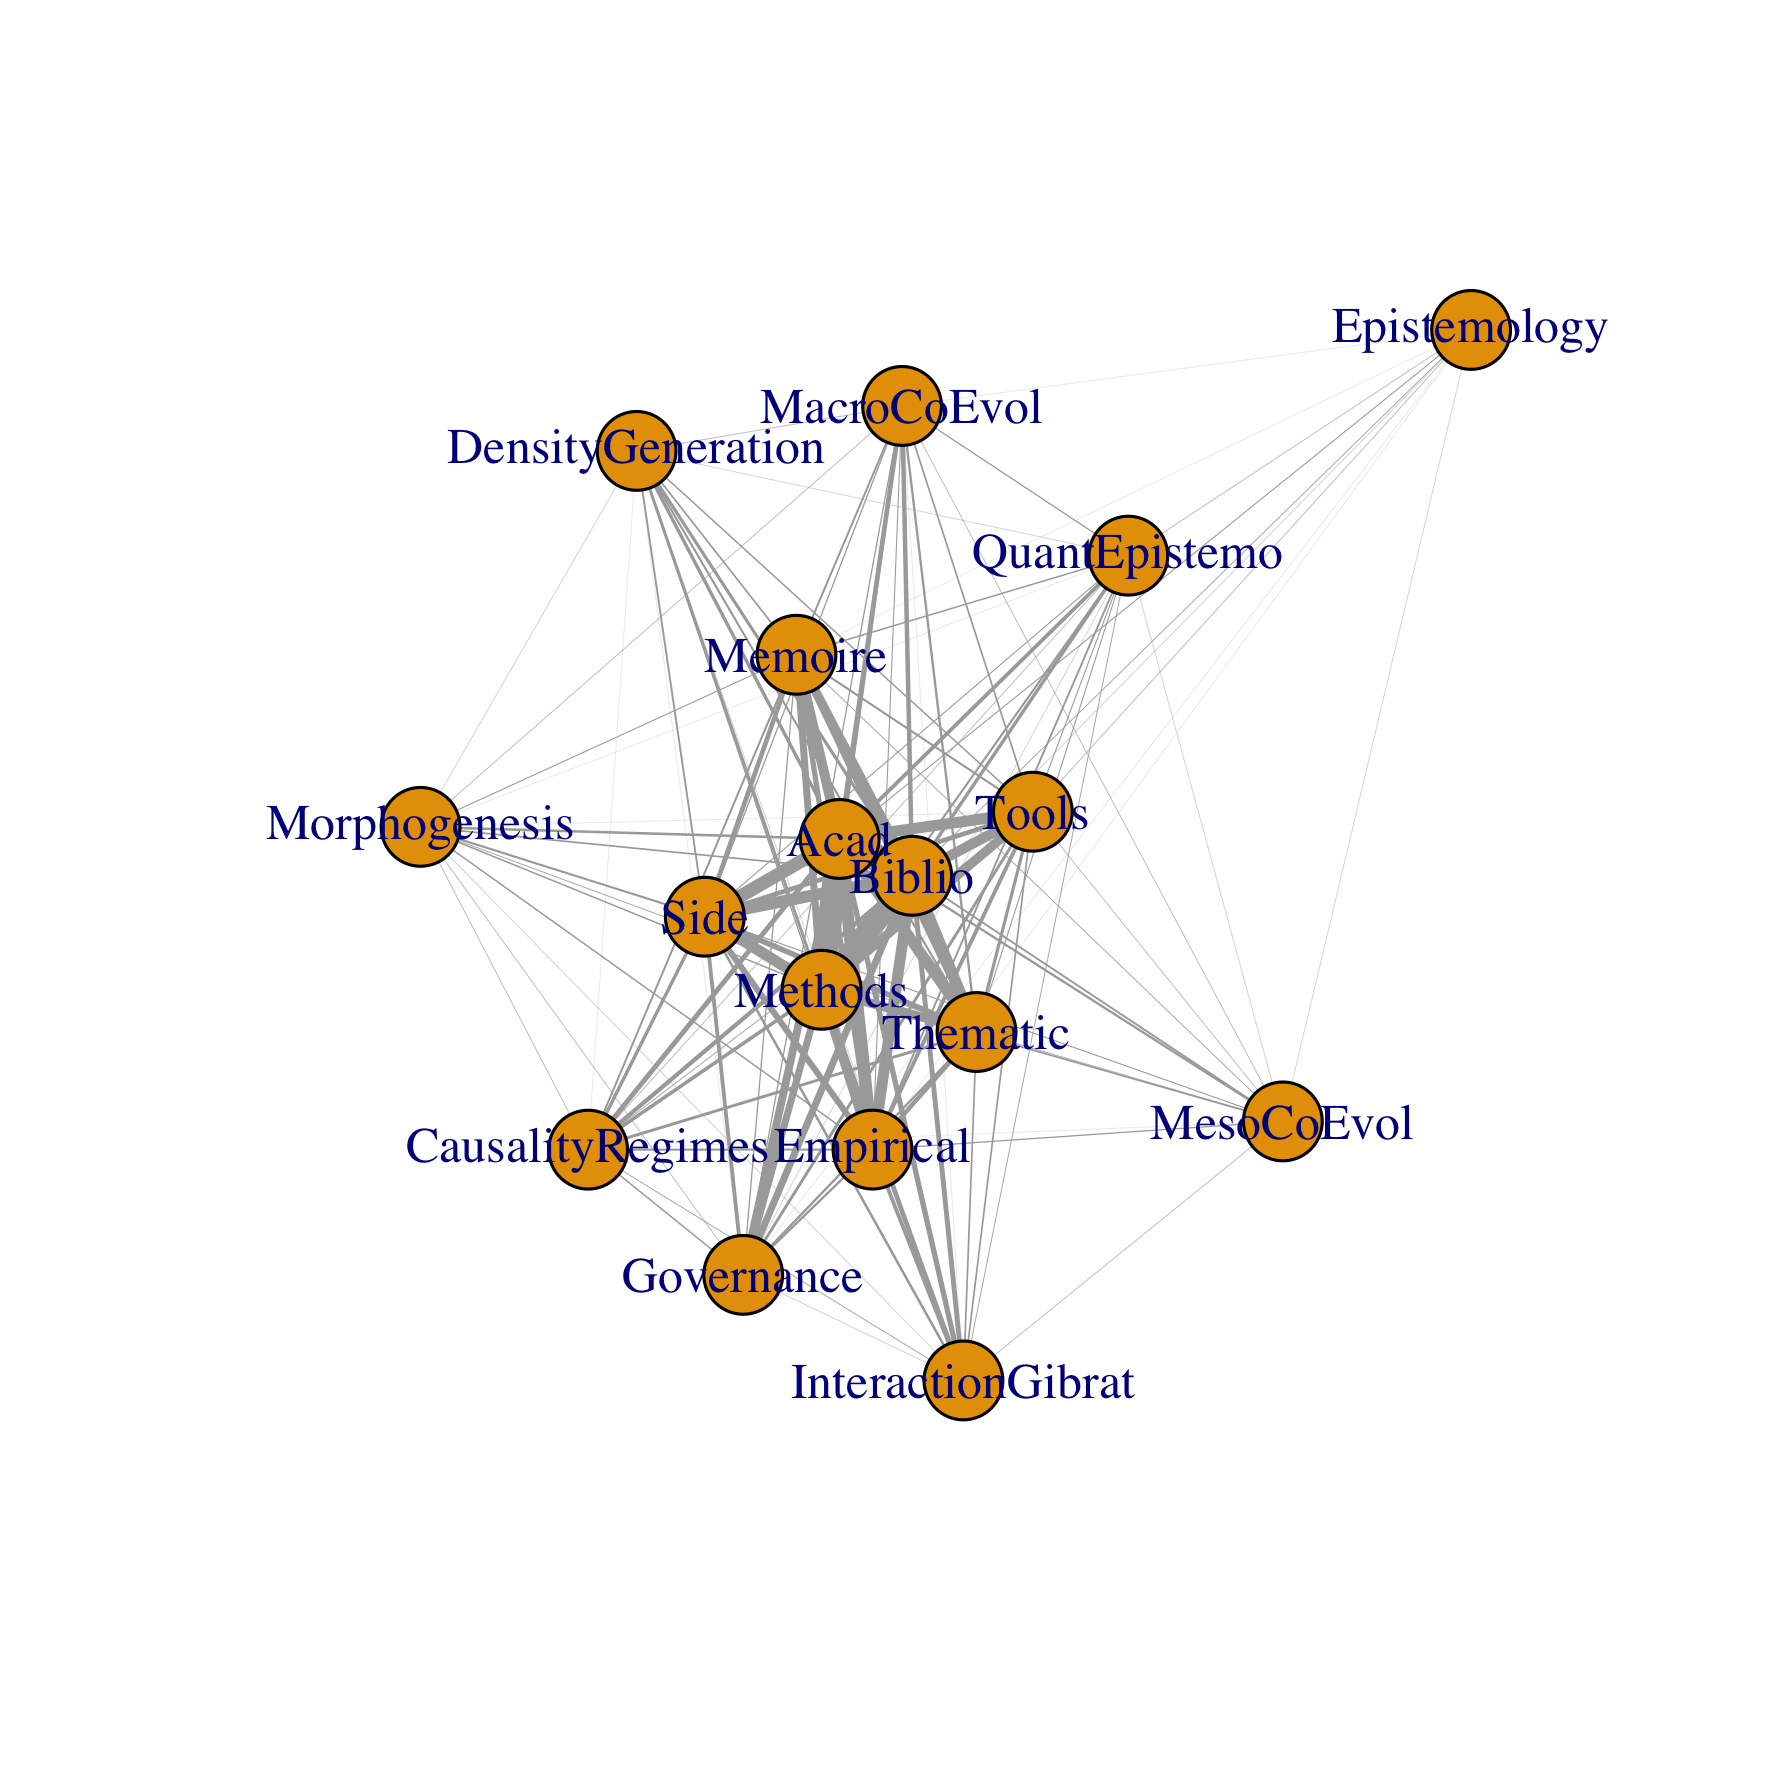
\includegraphics[width=0.49\linewidth]{Figures/Reflexivity/graph-projects-cooccs.png}
	%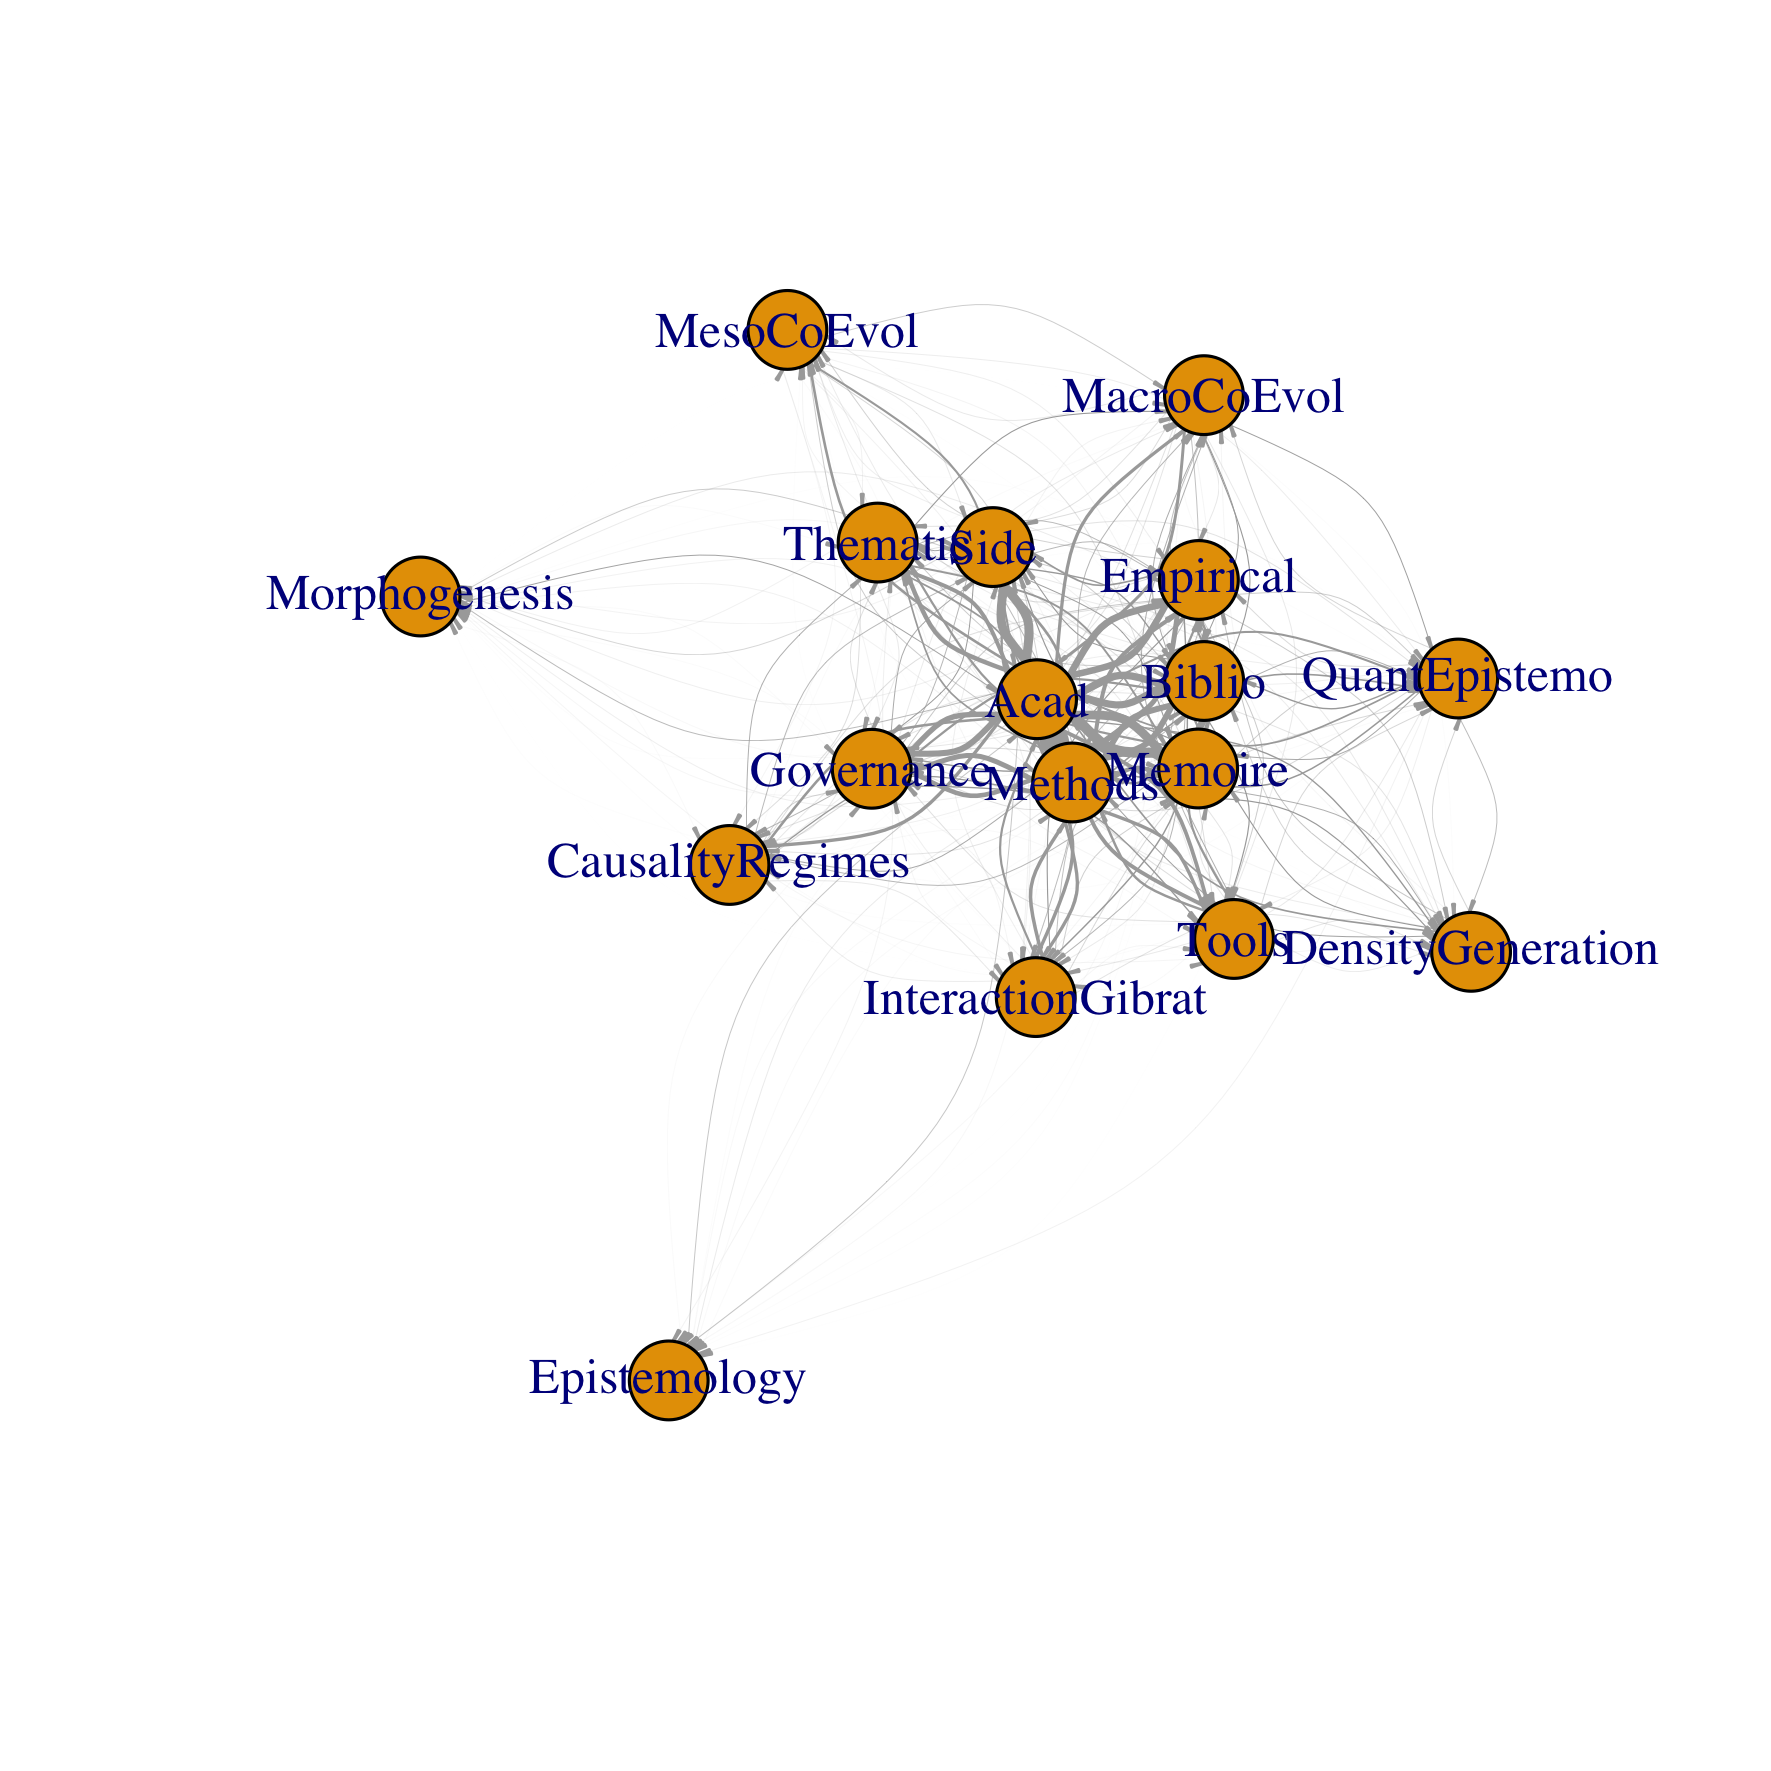
\includegraphics[width=0.49\linewidth]{Figures/Reflexivity/graph-projects-laggedflow.png}
	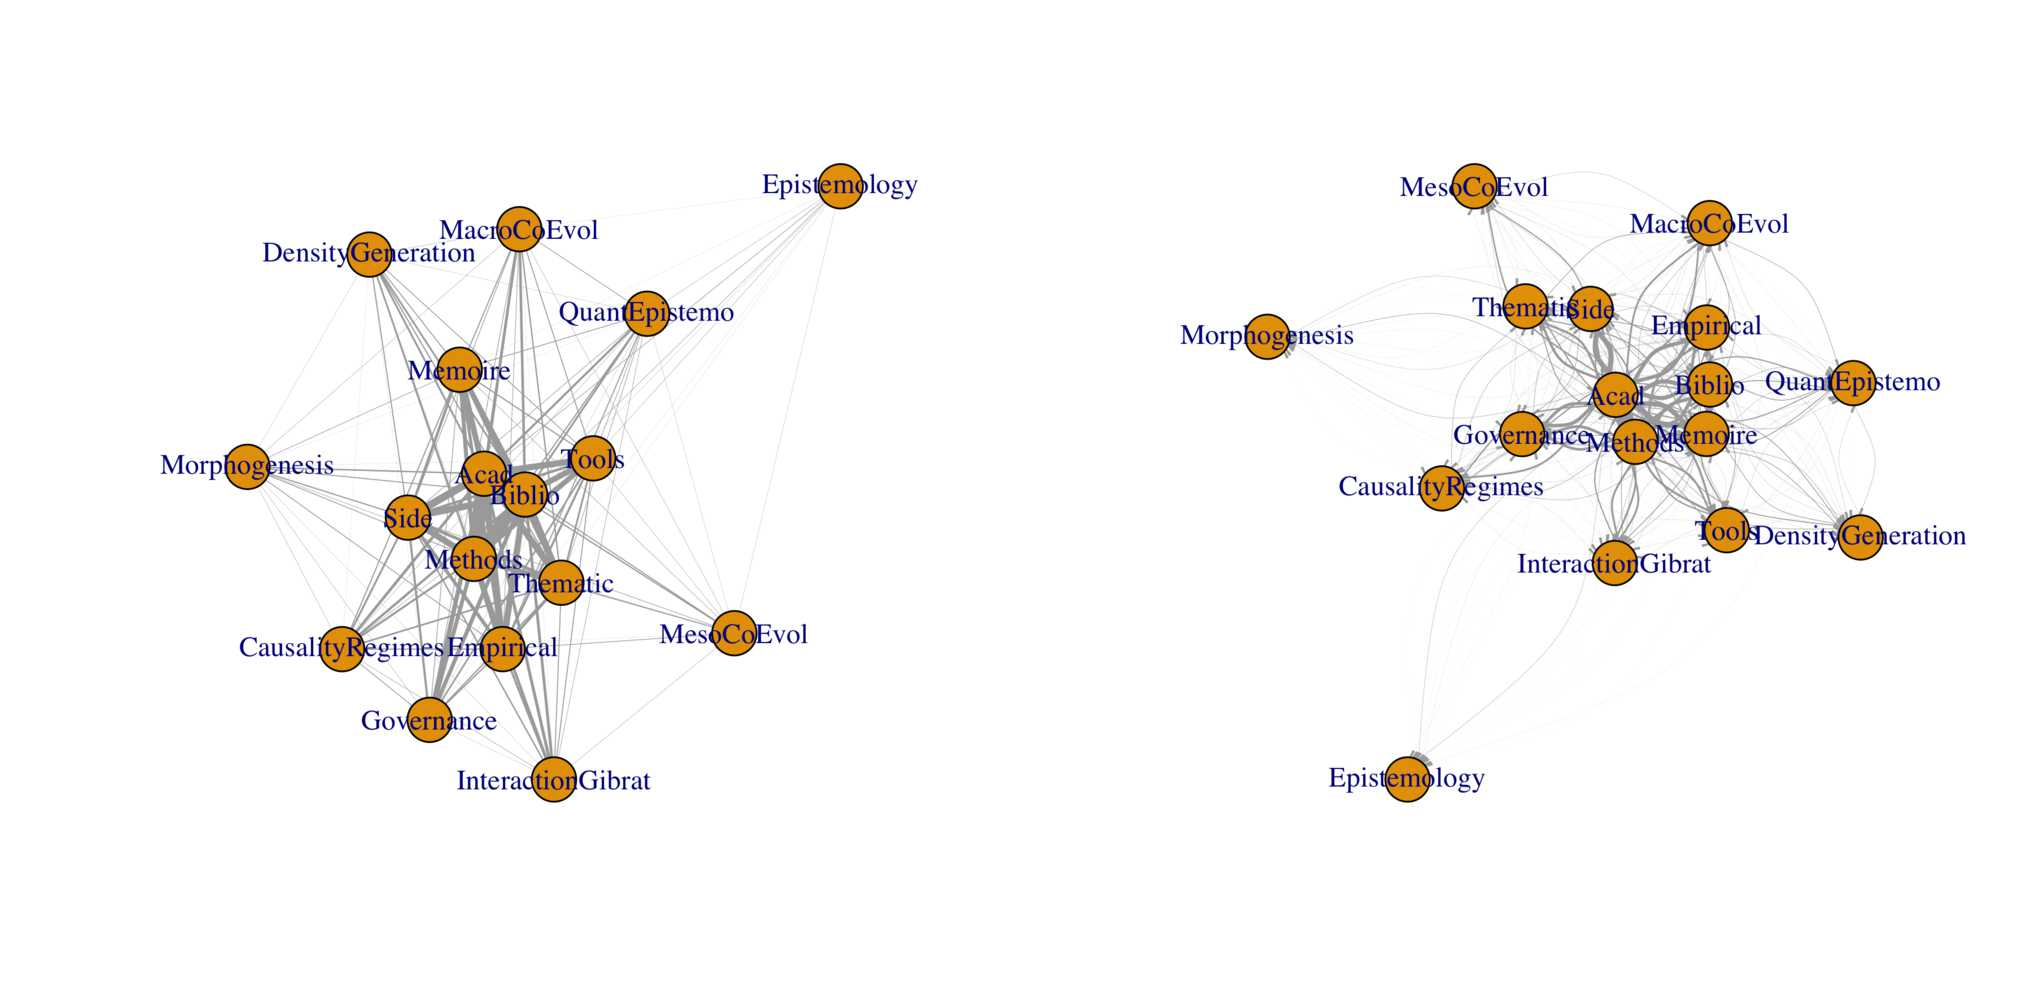
\includegraphics[width=\textwidth]{Figures/Final/F-reflexivity-projects.jpg}
	\appcaption{\textbf{Interaction networks between projects}\label{fig:app:reflexivity:projects}}{\textbf{Graphes d'interaction entre macro-projets.}\label{fig:app:reflexivity:projects}}
\end{figure}
%%%%%%%%%%%%



%%%%%%%%%%%%
\begin{figure}
	%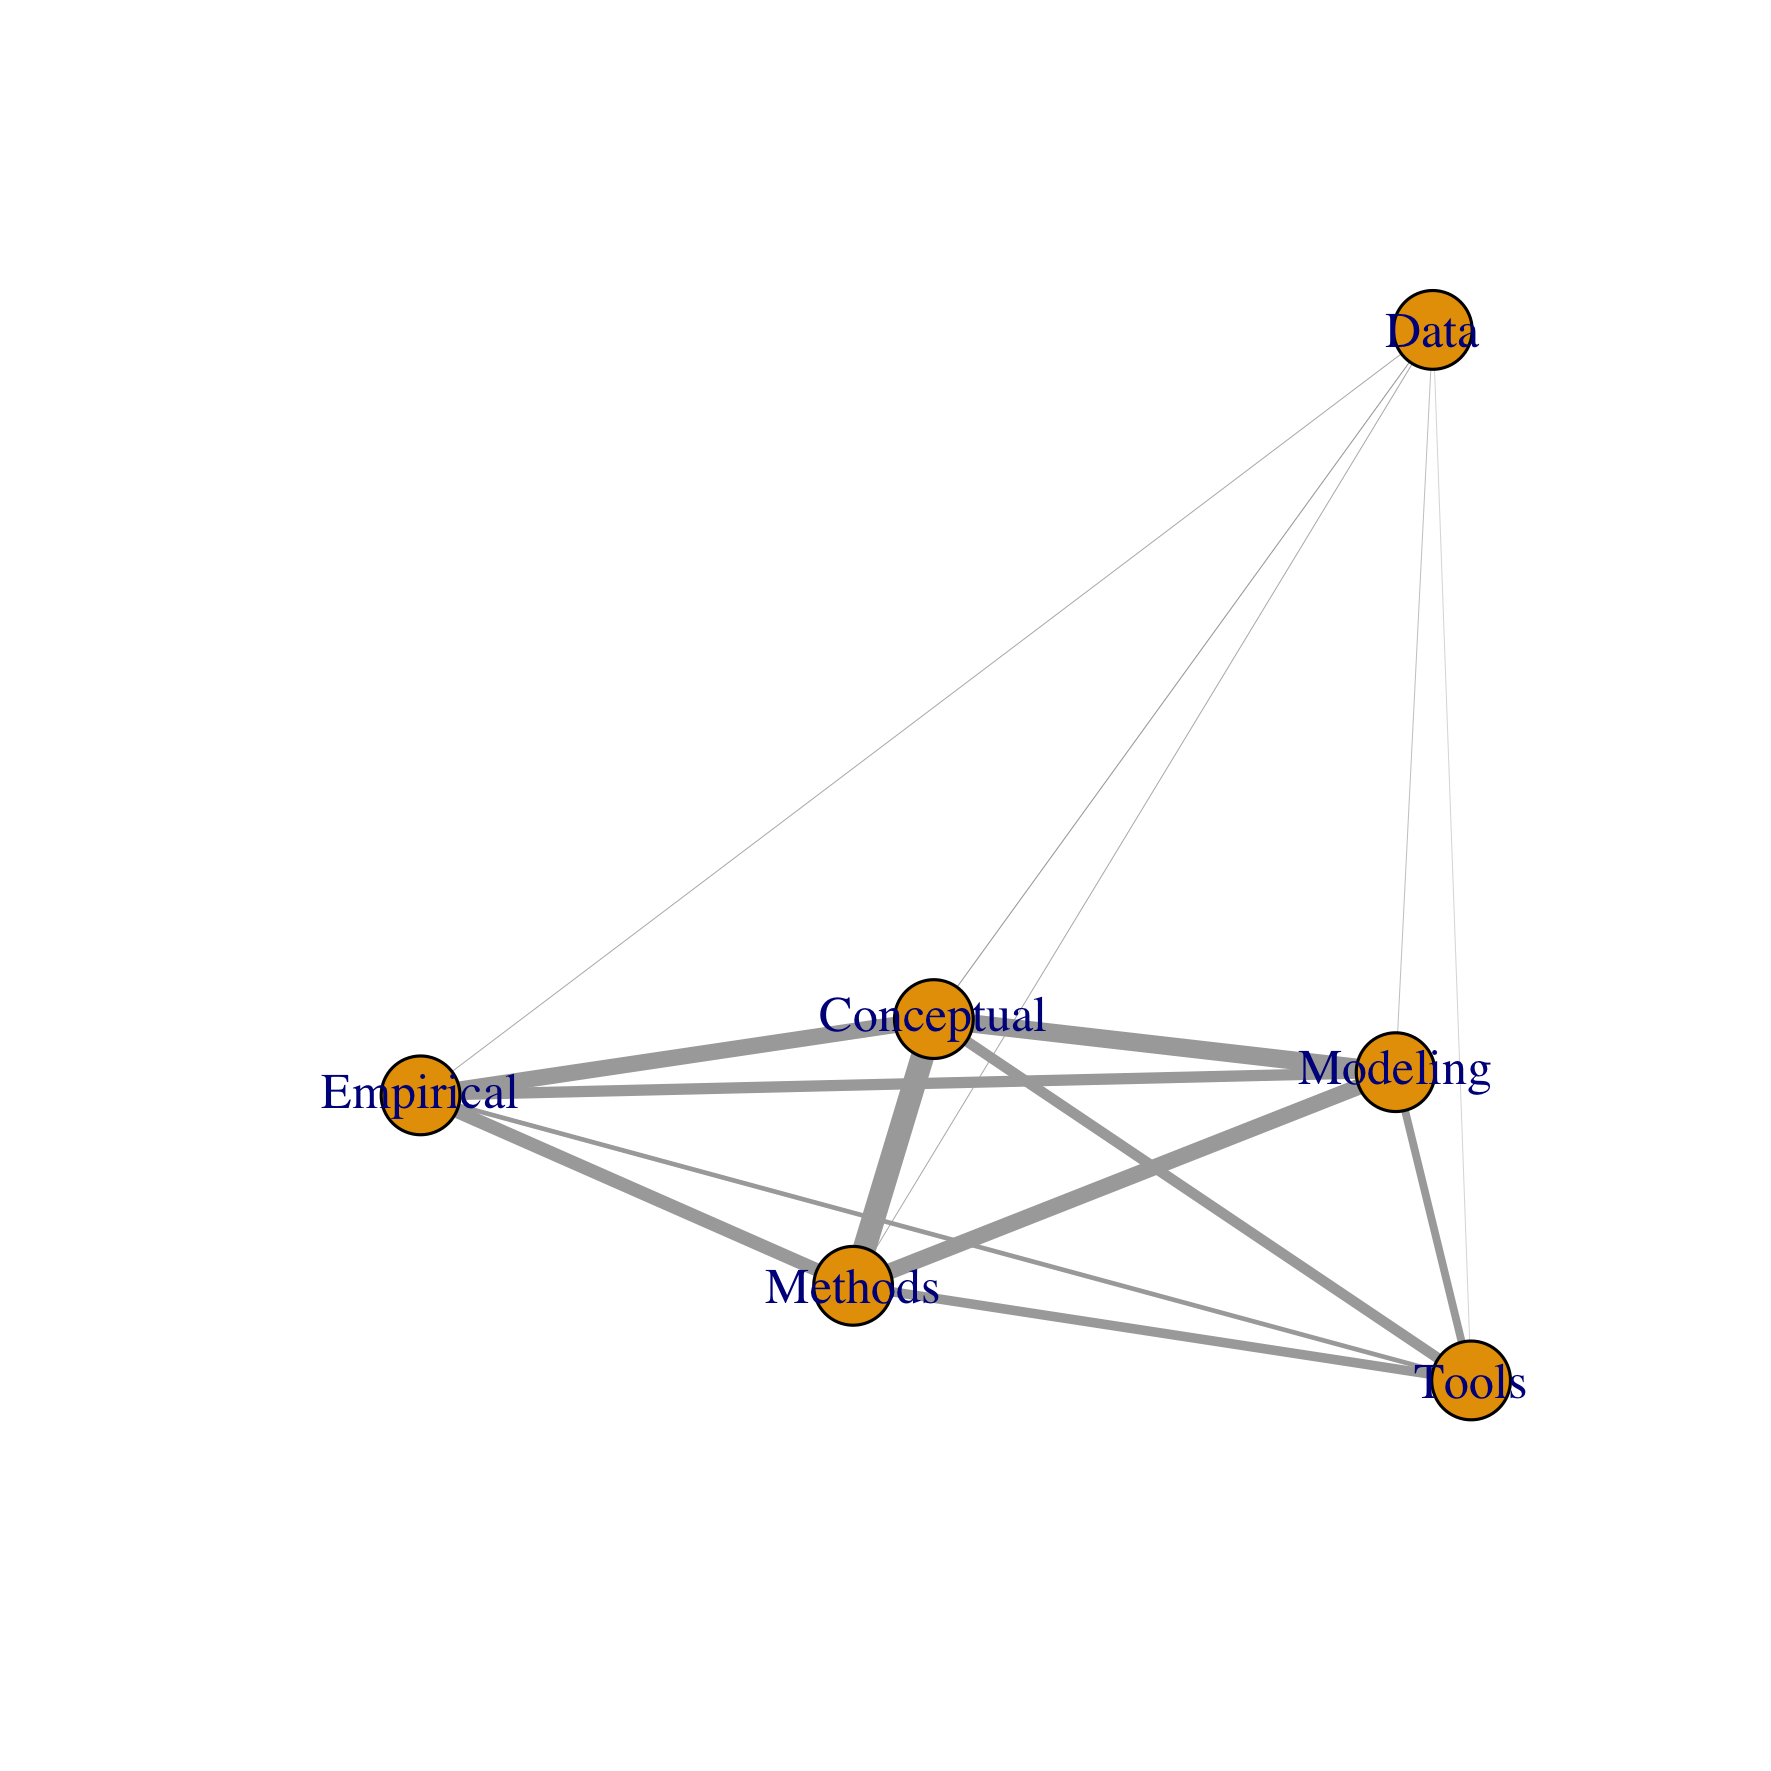
\includegraphics[width=0.49\linewidth]{Figures/Reflexivity/graph-kd-cooccs.png}
	%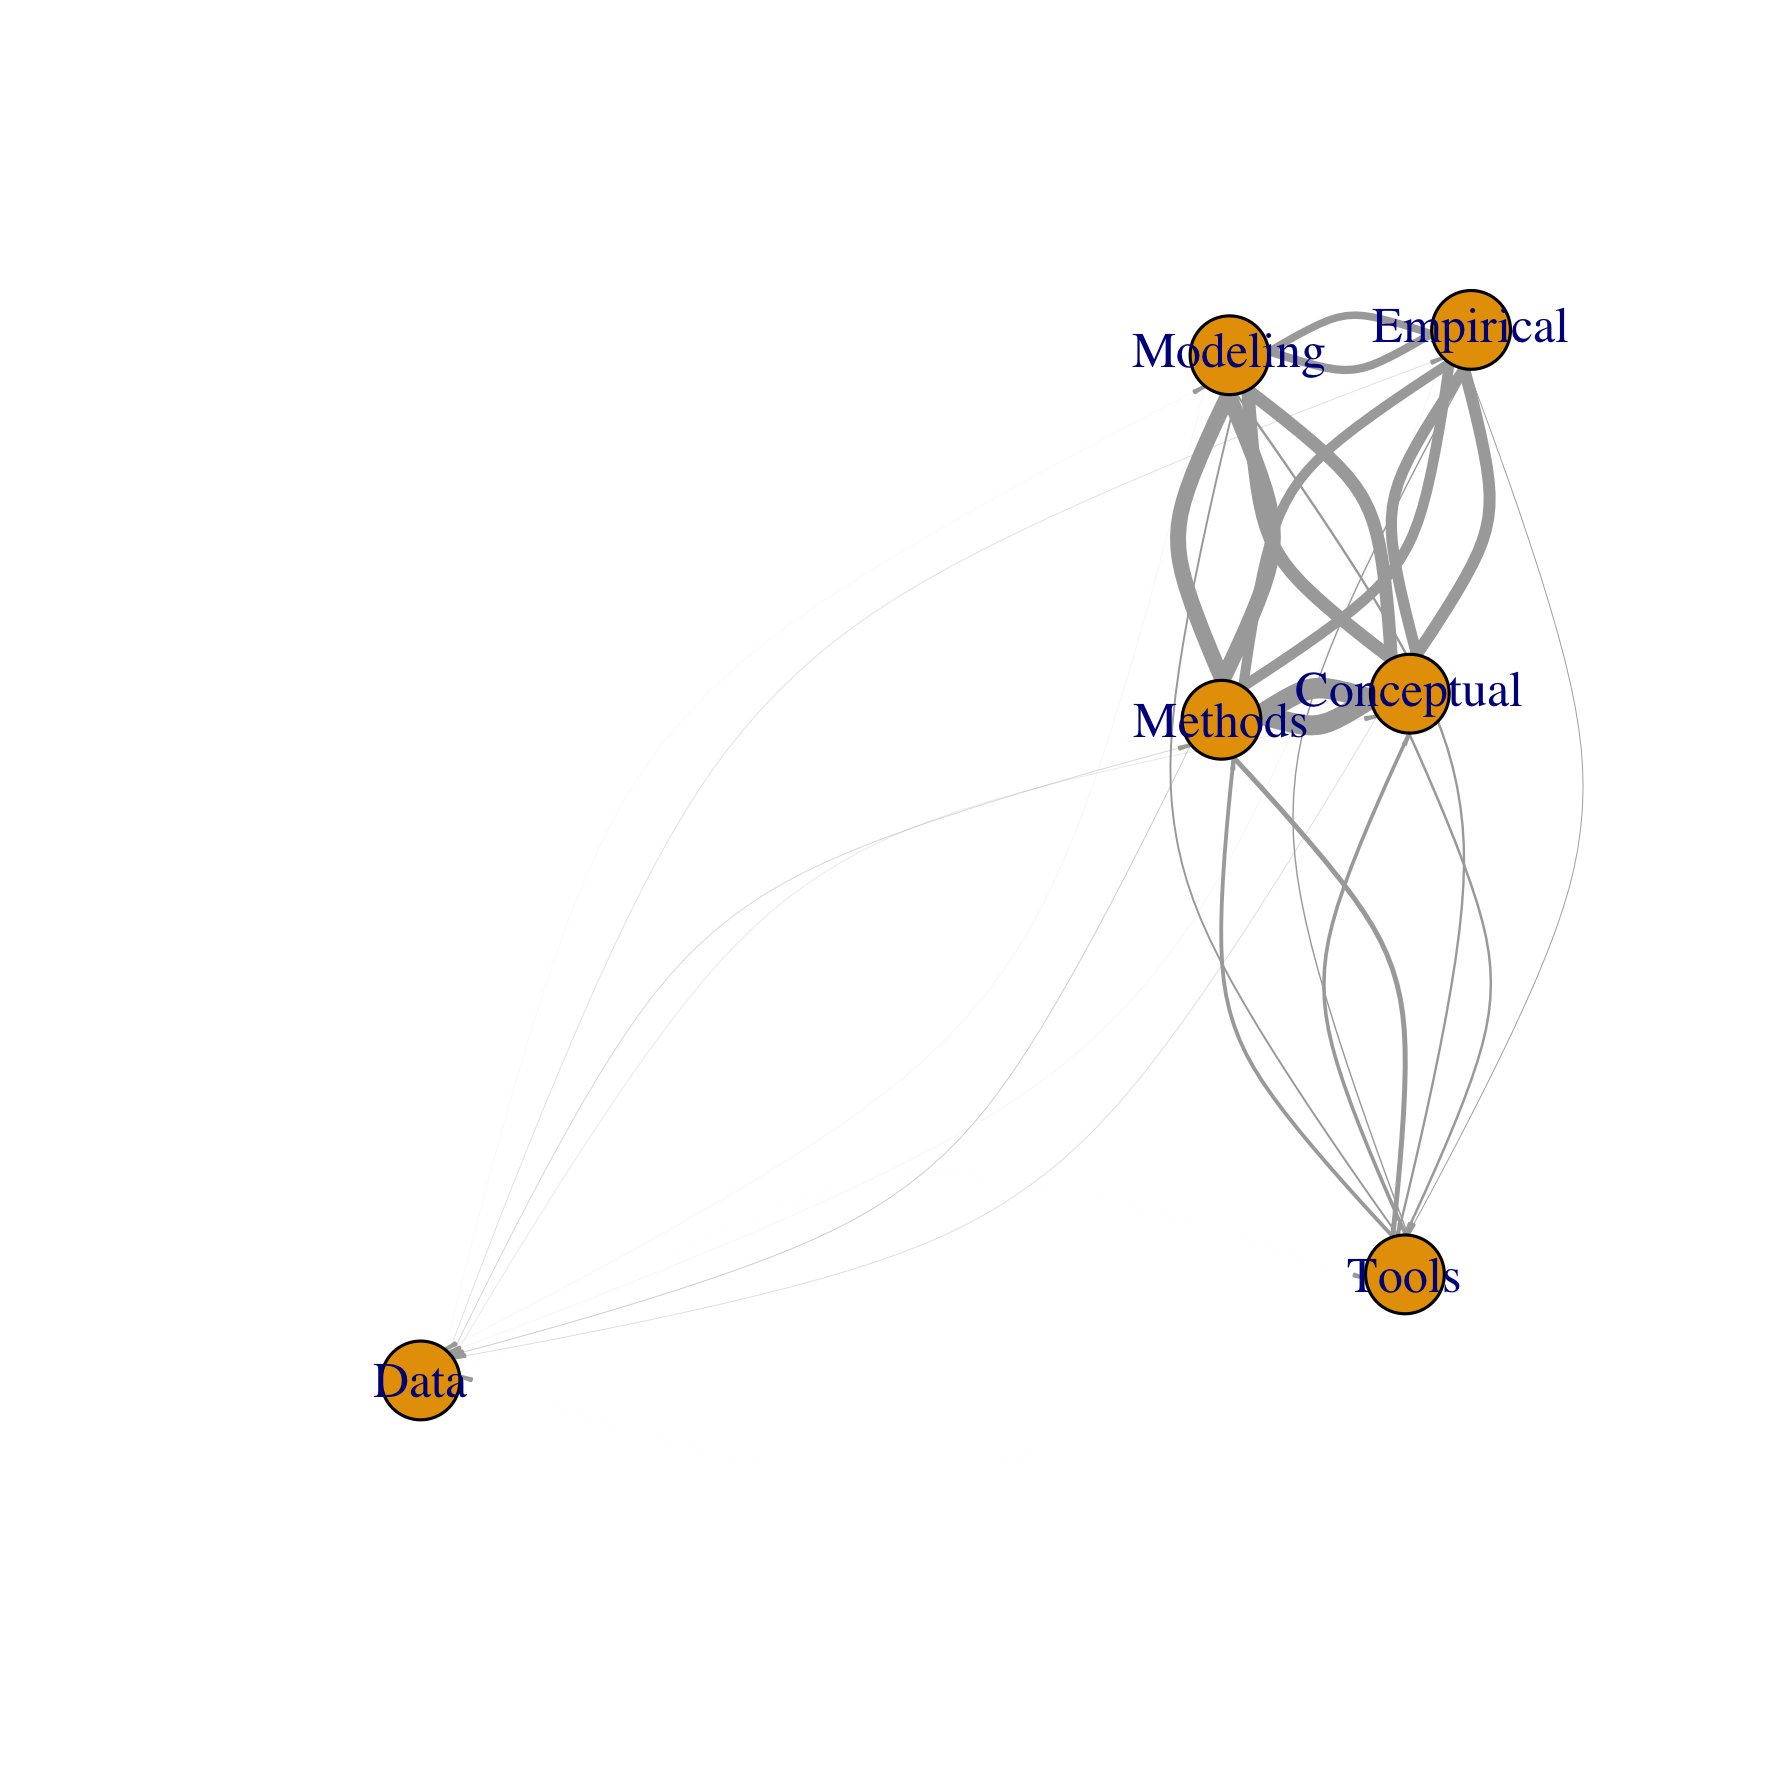
\includegraphics[width=0.49\linewidth]{Figures/Reflexivity/graph-kd-laggedflow.png}
	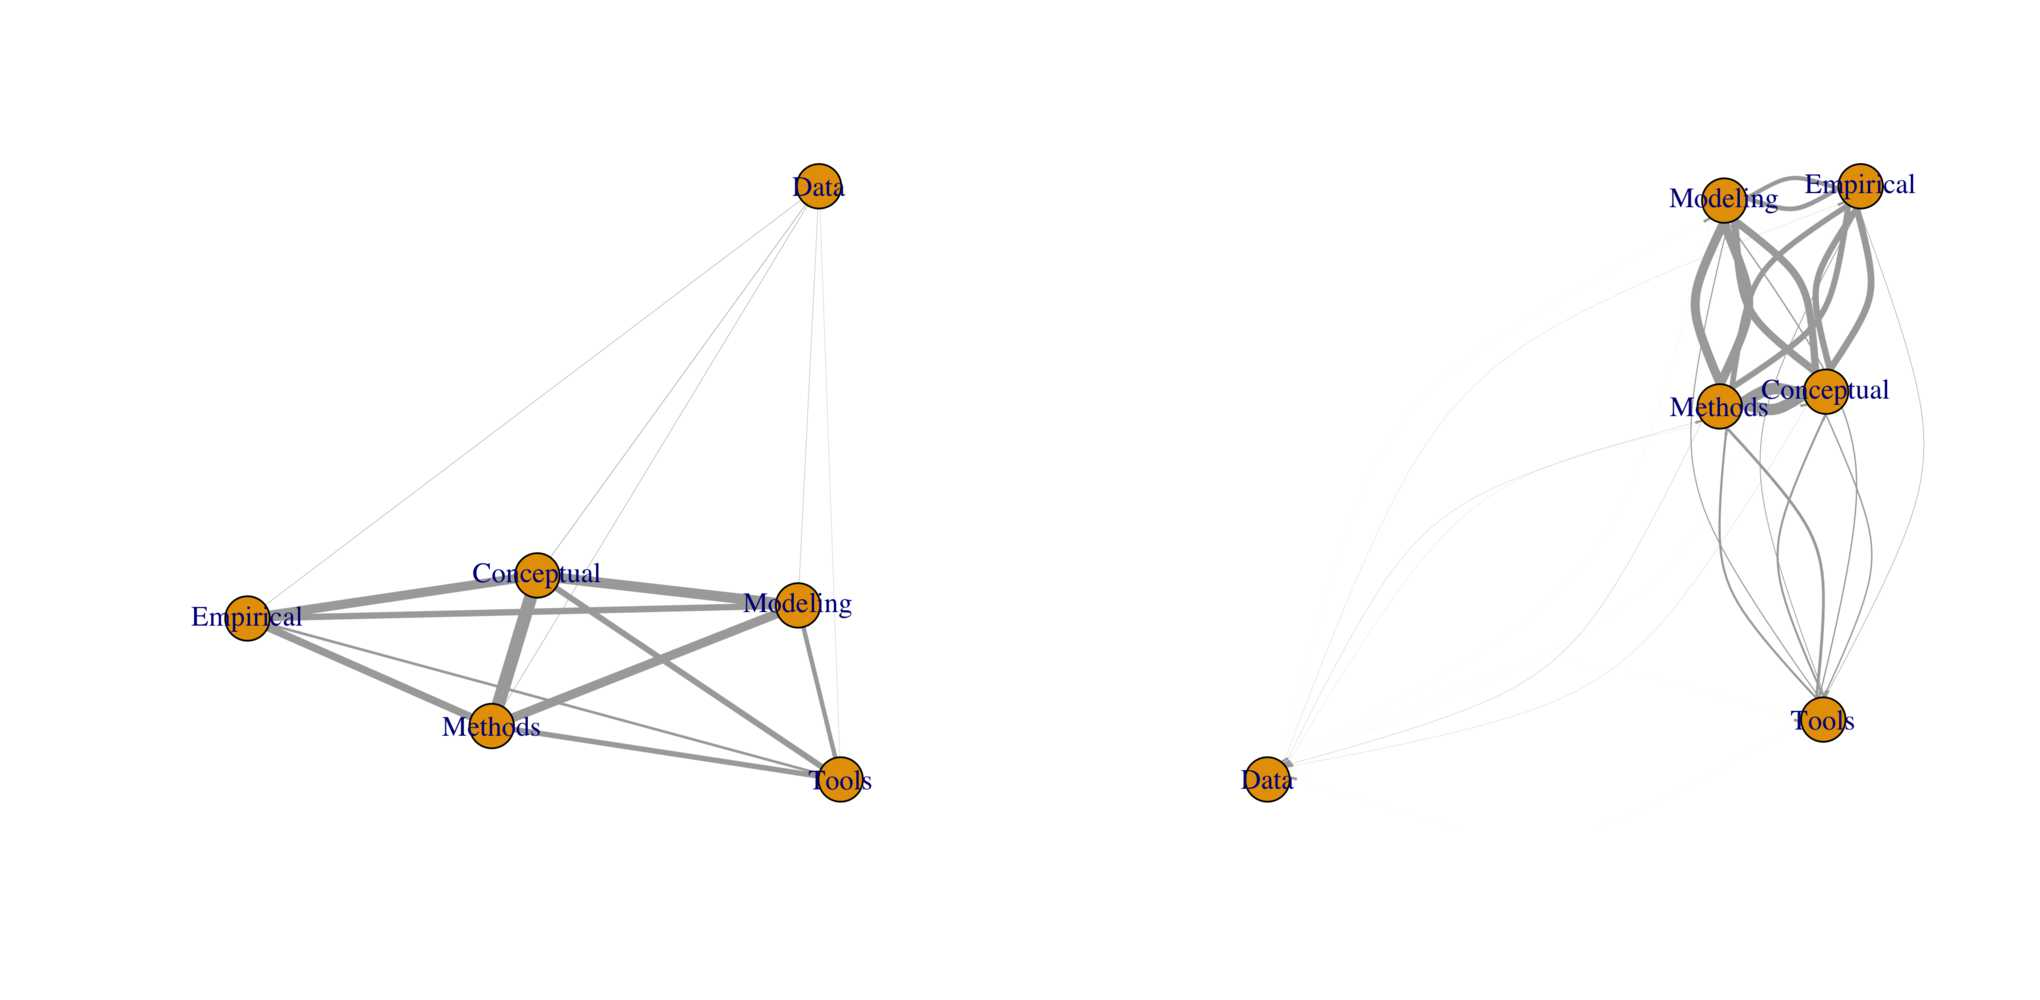
\includegraphics[width=\textwidth]{Figures/Final/F-reflexivity-kd.jpg}
	\appcaption{\textbf{Interaction networks between knowledge domains.}\label{fig:app:reflexivity:kd}}{\textbf{Graphes d'interaction entre domaines de connaissance.}\label{fig:app:reflexivity:kd}}
\end{figure}
%%%%%%%%%%%%






%%%%%%%
%% -- on hold --

%%%%%%%%%%%%
%\subsection{Concept maps}{Cartographie des concepts}

%concept maps : \cite{novak2008theory}

% faire un graphe des concepts ; compare to semantic network of concepts in Gödel Escher Bach.










